\documentclass[conference]{IEEEtran}

\usepackage{cite}
\usepackage{amsmath,amssymb,amsfonts}
\usepackage{graphicx}
\usepackage{textcomp}
\usepackage{multirow}
\usepackage{hyperref}
\usepackage{booktabs}
\usepackage{algorithm}
\usepackage{algpseudocode}
\usepackage{subcaption}
\usepackage{lipsum} % For lipsum
\usepackage[dvipsnames]{xcolor} % Custom Colors
\definecolor{mygray}{gray}{0.6} % Definining a .6 transparency gray called mygray
\setlipsum{% Making the lipsum text mygray
  par-before = \begingroup\color{mygray},
  par-after = \endgroup
}
\newcommand{\probP}{\text{I\kern-0.15em P}}
\newcommand{\tl}[1]{\textit{[{\color{red}#1}]}}
\newcommand{\cm}[1]{\textit{{\color{blue}#1}}}
\newcommand{\erik}[1]{\textit{[{\color{brown}Erik: #1}]}}
\newcommand{\mr}[1]{\textit{[{\color{brown}Mohammed: #1}]}}

\begin{document}

%%
%% The "title" command has an optional parameter,
%% allowing the author to define a "short title" to be used in page headers.
\title{A Tiny, Human-Interpretable, Client-Side, Classifier}

%%
%% The "author" command and its associated commands are used to define
%% the authors and their affiliations.
%% Of note is the shared affiliation of the first two authors, and the
%% "authornote" and "authornotemark" commands
%% used to denote shared contribution to the research.

\author{
    \IEEEauthorblockN{Charles Meyers}
    \IEEEauthorblockA{Umeå University\\
    % Umeå, Sweden\\
    \email{cmeyers@cs.umu.se}}
    
    \IEEEauthorblockN{Aaron P. MacSween}
 
    
    \IEEEauthorblockN{Tommy Löfstedt}
    % \IEEEauthorblockA{Umeå University\\
    % Umeå, Sweden\\
    % \email{tommy@cs.umu.se}}
    
    \IEEEauthorblockN{Erik Elmroth}
%     \IEEEauthorblockA{Umeå University\\
%     Umeå, Sweden\\
%     \email{elmroth@cs.umu.se}}
}

\maketitle

\begin{abstract}
  Machine learning have proven remarkable performance across a wide variety of domains, but nevertheless fail to adversaries during model training or deployment. 
  Recent developments have focused on incredibly complex architectures with long run-times, specific hardware requirements, and models that leak private information to anyone with access to the API.  
  However, the use of compression algorithms in conjunction with clustering algorithms has proven remarkably successful at text classification, excelling in few-show circumstances and across a wide-variety of datasets. This makes it ideal for a private anomaly detection algorithm. In this paper, we show how a client-side approach to anomaly detection is safer by design.
  In addition, we demonstrate the efficacy of this technique in the domain of computer security --- using datasets spanning computer processes, Twitter bots, intrusion attacks, denial of service attacks, and log file outlier detection.
  We offer advice for improving the model latency and evaluate NCD in the wider context of kernel metrics to show its broad efficacy.
\end{abstract}

\section{Introduction}

Despite their efficacy across many domains, modern machine learning methods often use very large models that require large numbers of samples to train~\cite{desislavov2021compute}. 
The exchange of this data often creates privacy and security risks~\cite{chakraborty_adversarial_2018,meyers}. For example, several attacks against ML systems have been proposed, targeting the model during training~\cite{biggio_poisoning_2013}, prediction~\cite{biggio_evasion_2013,deepfool,carlini_towards_2017}, or deployment~\cite{distributed_attacks,santos2021universal}. 
Even when access to a model is limited only to the classification labels, it is possible to subvert the model~\cite{hopskipjump}, reverse engineer the decision boundary~\cite{deepfool}, determine the model weights~\cite{jagielski2020high} or infer the class-membership of new samples~\cite{bentley2020quantifying}. 
This raises profound questions for safety critical systems~\cite{meyers} and legal questions about access and control of the underlying data~\cite{mitrou2018data,marks2023ai}. 
One solution to the problem of adversaries is to treat the model as we would treat a session token or any other private data --- by keeping it encrypted locally and providing no access in either direction to the internet. 
However, this lack of data sharing means that this hypothetical method must work well when trained on a small number of samples to minimise the run-time costs and maximise the efficacy for individual users. 
Recently, Jiang et al.~\cite{jiang2022less} proposed a parameter-free text classification algorithm (NCD-KNN) that exploits the distance measure \textit{normalized compression distance} (NCD) to classify objects using the NCD-nearest neighbours (KNN) algorithm.
This method has shown very strong performance against several benchmark datasets, but the choice of KNN over other simple models is seemingly unexplored and unjustified.
Therefore, we expand this concept of using NCD as a measure of distance to classifiers and compare their efficacy on anomalous datasets.
In this study, we explore the underlying theory of kernel methods, offer run-time improvements over Jiang's method~\cite{jiang2022less} and demonstrate the efficacy of our run-time optimised method on a variety of datasets.  


\subsection{Threat Model}
\label{threat}
A typical machine learning pipeline is vulnerable to attacks that target each stage of the machine learning pipeline. Broadly speaking, they come in white- and blacNCD-box categories~\cite{meyers}. Whitebox attacks like the fast gradient method~\cite{fgm} or~\cite{deepfool} require access to the model directly while other attacks can succeed with only normal . However, it has been shown that this finding prototypical meta samples from the training set is trivial~\cite{chakraborty_adversarial_2018}. Likewise, we can then use this class membership data to reverse engineer the model weights~\cite{} and loss gradients for a set of (potentially adversarial) examples~\cite{}. Even if our attacker only has access to a typical application programming interface (API), there are effective adversaries~\cite{hopskipjump}. In short, the model-as-a-service paradigm is inherently fragile to attackers and dangerous for user privacy. Instead of relying on a model trained on massive amounts of user data, as is typical in deep neural networks and other ``big data" approaches, we can categorically sidestep these attacks with a model that runs entirely client-side. By avoiding the typical model-as-a-shared service approach, the attack surface is reduced to only adversaries that have access to data that users generally consider private (e.g. the contents of a message). That is, the attack surface is reduced to that of any other cookie or browser-based secret~\cite{} and cab be unique to each user, session, or device.

\subsection{Motivations} 
We have several motivations for this work. 
First, \textit{normalized compression distance} (NCD) has been demonstrated to be a \textit{universal} measure of similarity between two objects~\cite{ncd}.
Secondly, Jiang's analysis relies on many thousands of samples and it's unclear how well it performs in the few-shot circumstances or in the case of extremely imbalanced data. 
While follow-up research examined topics like image classification~\cite{opitz2023gzip}, chemical classification~\cite{weinreich2023parameter}, and text classification~\cite{nishida2011tweet}, it has not been explored in the context of anomaly detection to the best of our knowledge.
Thirdly, we can expand 
Furthermore, if we can minimise the run-time storage and computation requirements, then we can fulfill our goal of deploying this method entirely client-side.
In the simplest case, that might mean marking an email as spam~\cite{} or examining the nearest neighbours in a browser~\cite{}. Rather than writing another paper about large language models~\cite{} or deep convolutional networks~\cite{} in 2024, the goal of this work is to convince at least one reader that they probably don't need one.
 

\subsection{Contributions}
In this study, we:

\begin{itemize}
    \item explore the theory behind normalized compression distance as a pseudo-metric,
    \item demonstrate how private model deployment is safer by design(Sec.~\ref{threat}),
    \item offer run-time improvements over the NCD-KNN classifier (Sec.~\ref{improvements}),
    \item provide a \texttt{javascript} as well as a \texttt{scikit-learn} implementation,
    \item demonstrate the efficacy of the NCD-KNN classifier across several anomaly detection datasets,
    \item and demonstrate the efficacy of the run-time optimisations.
\end{itemize}





\section{Background}

In the sections below, we outline the definition of a metric space and the connection to normalized compression distance, briefly k-Nearest Neighbor (KNN) classifiers, and give a high-level overview of the gzip compression algorithm.

\subsection{Measures of Distance}
There are many different distance measures. Jiang et al. examined only the noise-compression distance (see Sec.~\ref{ncd}), but this method is identical to other classifiers~\cite{vapnik1994measuring} that use measures of distance to cluster samples into classes. For strings, several measures of distance are routine and available via the \texttt{levenshtein} package~\cite{levenshtein}. The set of evaluated string metrics is outlined in Sec.~\ref{string_metrics}.





\subsubsection{Normalized Compression Distance}
\label{ncd}
The normalized compression distance (NCD) is defined as:
\begin{equation}
    \text{NCD}(x, y) = \frac{\mathcal{C}(xy) - \min[\mathcal{C}(x), \mathcal{C}(y)]}{\max[\mathcal{C}(x), \mathcal{C}(y)]} + \varepsilon,
\end{equation}
where $\mathcal{C}(z)$ is the length (in bits) of the compressed form of the data $z$ using a compression algorithm (\textit{e.g.} DEFLATE), $xy$ denotes the concatenation of strings $x$ and $y$, and $\varepsilon$ is an error term~\cite{ncd}. It is generally assumed to to be small relative to the rest of the terms and the original authors denote that it can yield values larger than one~\cite{ncd}. To the best of knowledge of the authors, nobody has addressed the problem of negative values for NCD\@.
Nevertheless, it has been used for classification tasks many times~\cite{opitz2023gzip,weinreich2023parameter,nishida2011tweet,jiang2022less} where the error term is simply assumed to be irrelevant. 
We discuss novel mitigation techniques in Section~\ref{pseudometric} and the effect of these mitigation techniques is examined in Figures~\ref{fig:mod_assumptions}~and~\ref{fig:mod_acc}.

\subsubsection{Other measures of string distance}
\label{string_metrics}
In addition to the NCD metric defined above, we examined several other measures of string similarity, widely used in natural language processing (NLP) and these are briefly outline below. 
% String Distances
\begin{itemize}
    \item \textit{Levenshtein:} the "edit distance" or minimum number of single-character edits to transform one string into another~\cite{navarro2001guided}.
    \item \textit{Ratio:} is one minus Levenshtein distance divided by the total length of the strings~\cite{levenshtein}.
    \item \textit{SeqRatio:} identical to "Ratio", but calculated on sequences of strings by taking the single input string and splitting it into a list around white-space characters~\cite{levenshtein}.
    \item \textit{Hamming:} is the number of character positions where two strings differ, but is only defined for strings of equal length, leading to sparse distance matricies~\cite{hamming_distance}.
    \item \textit{Jaro:} is a measure of similarity between two strings, taking into account the number of identical characters as well as the number of transposed characters~\cite{jaro}.
    \item \textit{Jaro-Winkler:} extends the above by incorporating a scaling factor to give weight to sub-strings that occur more frequently~\cite{jaro}. 
\end{itemize}



\subsubsection{Metric Spaces}

A metric space is defined as some measure of distance between the constituent components of some space, usually called points.  For points $x_1,x_2...x_n \in X$ in a metric space, separated by distance $d(x_1,x_2)$, $d$ is a proper metric if and only if the following 4 identities are true~\cite{metrics}, each of which is given a label (which we've denoted in the parentheses):

\label{metric_spaces}
\begin{itemize}
    \item $d(x_1,x_2) = 0 \iff x = y$ (zero identity)
    \item $d(x_1,x_2) \geq 0$ (non-negativity identity)
    \item $d(x_1,x_2) = d(y, x)$ (symmetry identity)
    \item $d(x_1, x_3) \leq d(x_1,x_2) + d(x_2,x_3)$ (triangle inequality).
\end{itemize}
This metric space is often given the notation $M(X,d)$ since it is defined by the set, $X$, and the distance function, $d$.
In addition, we use the following notation to denote an inner product
$$
\langle \cdot , \cdot \rangle : V \times V \rightarrow \mathbb{R}
$$

for a vector space, $V$, and the field of real numbers, $\mathbb{R}$. 
Vector spaces, by definition are, at least, positive semi-definite such that for any (real-valued)vector, $X$, 
\begin{equation}
\langle X, X \rangle \geq 0
\label{eq:psd}
\end{equation}

\subsubsection{Mercer's Theorem and Kernelisation}
\cm{This is here because I'm still running the rbf(ncd(x,y))}
Whereas distance functions are used to measure the similarity between different examples $x,y$, a \textit{kernel-function}, $K$, is a measure of similarity. That is, when $d(x_1,x_2) = 0, x = y$ , but when $K(x_1,x_2) = 0, x~\perp~y$. The opposite then follows when $d(x_1,x_2)=1$ or $K(x_1,x_2)=1$. Mercer's theorem says that for any symmetric, continuous function, $K$,
$$
K : [a, b] \times [a, b] \rightarrow \mathbb{R}~\forall~x_1,x_2 \in [a,b].
$$
$K$ is said to \textit{positive semi-definite} if and if only for any set of points, $\{x_1, x_2, \cdots x_n\}$, and any set of real numbers, $\{ c_1, c_2 \cdots c_n\}$, then
\begin{equation}
\sum_{i=1}^n \sum_{j=1}^n K(x_i, x_j) c_i, c_j \geq 0.
\label{eq:mercers_theorem}
\end{equation}
That is to say, Equations~\ref{eq:psd}~\&~\ref{eq:mercers_theorem} are equivalent statements when 
$$
K(x_1, x_2) = \langle \phi(x_1), \phi(x_2) \rangle \nu
$$
where $\nu$ is the feature vector space and $\phi(\cdot)$ is a function that extracts features from $x_1,x_2$.


\subsection{Calculating the Gram matrix}
\label{gram_matrix}
While many of the above distance metrics are symmetric, this is not-necessarily the case with NCD and this matrix must be calculated for all pairs of samples $x_i, x_j~\forall~x_i,x_j \in X_1, X_2$. 
That is to say, the run time scales with the magnitude ($ || \cdot || $) of sets, denoted $n = || X_1 ||, m = || X_2 ||$, such that the run time is $\mathcal{O}(n,m)$ for both compute and memory.
\begin{algorithm}
    \begin{algorithmic}
        \Require datasets $X_1$, $X_2$ and some distance function $d(x,x)$.
        \For{$x_i \in X_1$}
            \For{$x_j \in X_2$}
                \State $D_{ij} \gets d(x_i, x_j)$
            \EndFor
        \EndFor
        \State \Return Gram matrix $D$ with dimensions $i,j$.
    \end{algorithmic}
    \caption{Compute the ``Vanilla'' Gram matrix}
    \label{alg:vanilla}
\end{algorithm}

% However, using the \textit{kernel trick}, we can change this distance matrix into a kernel matrix \cite{}.
% The main effect of this is that we can turn the prediction step from this $\mathcal{O}(n,m)$ t
%For some square matrix (e.g. $n=m$), $A$, the trace function, $\mathbf{tr}(\cdot)$ is defined as the sum of the diagonal entries in the matrix ($a_{i,i} \in A$), such that
% $$
% \mathbf{tr}(A) = a_{1,1} + a_{2,2} \cdots a_{n,n}.
% $$
% For square matrices with the same dimensionality $A,B$, the trace function is known to have the following properties:
% \begin{align*} 
% \mathbf{tr}(A, B) &= \sum_{i=1}^{n} \sum_{j=1}^{m} A_{i,j} B_{i,j} \\
%                   &= \mathbf{tr}(A^T B) \\
%                   &= \mathbf{tr}(B^T A) \quad \text{(cyclic property of the trace)} \\ 
%                   &= \langle A, B \rangle_F \quad \text{(Frobenius inner product)} \\
%                   &= \sum_{i=1}^{n} \sum_{j=1}^{m} A_{i,j} B_{i,j} \quad \text{(element-wise product)} \\
%                   % &= \sum_i{i=1}^n \lambda_i (A) \lambda_i(B) additional
%                   &= K(X_1, X_2) \quad \text{(Kernel function)}.
% \end{align*}
% That is, if NCD can be forced to adhere to the constraints outlined in Section~\ref{metric_spaces} and Equations~\ref{eq:psd}~\&~\ref{eq:mercers_theorem}, then the run time can be reduced from $\mathcal{O}(nm) = O(n^2)$ to $\mathcal{O}(n)$. 
Clearly, if the number of training samples is large, compressing a text message thousands of times to make a prediction, clearly becomes infeasible. 
One approach is to find the most important training samples and discard the rest before the prediction step, which is known as sample \textit{condensing}~\cite{}.
There are many known techniques for this, some of which are outlined in Section~\ref{condensing_methods}.


\subsection{KNN}
\label{runtime}
The algorithm for KNN is reproduced in Algorithm~\ref{alg:knn}. As we can clearly see, this scales with the size of the training set $m = || X_{\text{train}} || $ as well as the test set, $n = || X_{\text{test}} ||$, giving a run-time of $\mathcal{O}(mn)$.
This makes it unsuitable for real-time classification when there are many training samples. 
Furthermore, if we would like to add weights to the samples (as in a weighted KNN) or use another algorithm like logistic regression or support vector classifiers (SVCs), then training consists of find the distance matrix $D_{i,j} = d(x_i, x_j) \forall i,j \in X_{\text{train}}$, yielding a run-time of $\mathcal{O}(m^2)$ for training and $\mathcal{O}(mn)$ for inference. Strategies for overcoming this limitation are discussed and evaluated below (see: Sections~\ref{condensing_methods}~and~\ref{condensing}, and Figure~\ref{fig:condense_summary}). 



\begin{algorithm}
\begin{algorithmic}
    \caption{``Vanilla'' KNN Classifier}
    \label{alg:knn}
    \Require{
        \\training data, $x_i \in X_{\text{train}}$;
        \\training labels, $y_i \in Y_{\text{train}}$;
        \\test set, $x_j \in X_{\text{test}}$;
        \\distance function, $d(x_1,x_2)$;
        \\sorting function, $S(X)$;
        \\voting algorithm, $V(X)$;
        \\number of neighbors, $k$.
    }
    \State $D \gets d(x_i,x_j) \forall \left( x_i \in X_{\text{train}}, x_j \in X_{\text{test}} \right)$ \Comment{Algorithm~\ref{alg:vanilla}} 
    \For{$x_j \in X_{\text{test}}$}   \Comment{KNN}
        \State $I_j \gets S(D_{*,j})$ \Comment{Get sorted indices of neighbors}
        \State $N_j \gets I_j[0 \ldots k-1]$ \Comment{Get first k indices}
        \State $Y_j \gets V(Y_{\text{train}}[N_j])$ \Comment{Get the majority class}
    \EndFor
    \State \Return $Y_{\text{test}}$
\end{algorithmic}
\end{algorithm}




\subsection{NCD-KNN}
\label{ncd-knn}

A recent popular introduced NCD as a ``parameter-free'' measure of distance for the KNN classifier~\cite{jiang2022less}, though NCD as a measure of distance dates back two decades~\cite{ncd}. 
To use NCD as a measure of distance, one must choose a compression algorithm. This has been explored, in part, before ~\cite{ncd_pitfalls}, but we expand their analysis to newer compression algorithms and offer additional run-time improvements.
In addition to GZIP, we tested LZMA, BZ2, and ZSTD. A summary of the tested compressors can be seen in Table~\ref{tab:compression_algorithms}.

\begin{table*}[h]
    \centering
    \caption{Comparison of Compression Algorithms for NCD-KNN. \cm{TODO: Add citations}}
    \begin{tabular}{|c|c|c|c|c|l|}
        \hline
        \textbf{Algorithm} & \textbf{Compression Ratio} & \textbf{Compression Speed} & \textbf{Memory Usage} & \textbf{Complexity} & \textbf{Description} \\ \hline
        GZIP  & Moderate & Fast & Low  & Low & LZ77 and Huffman coding. \\ \hline
        LZMA  & High     & Slow & Moderate & High & Lempel-Ziv with range encoding. \\ \hline
        BZ2   & High     & Moderate & Moderate & Moderate & Burrows-Wheeler and Huffman coding. \\ \hline
        ZSTD  & Very High & Very Fast & Low & Moderate & LZ77 algorithm with high-speed entropy coding. \\ \hline
        Brotli & High & Fast & Moderate & Moderate & LZ77 with context modeling and Huffman coding. \\ \hline
    \end{tabular}
    \label{tab:compression_algorithms}
\end{table*}

However, there are some cases that are not covered, particularly when the strings are very short or the alphabet is very small (see: Section~\ref{pseudometric} and Figure~\ref{fig:mod_assumptions}).
Section~\ref{pseudometric} details these edge cases and Section~\ref{improvements} details the proposed mitigations and improvements.
The results in section~\ref{results} show how this modified NCD algorithm has no negative effect on the accuracy while reducing the number of calculations required to the Gram matrix by a factor of two.  



\section{NCD is a pseudo-metric}
\label{pseudometric}
While NCD is often discussed as a measure of distance, it doesn't always follow the formalized constraints of proper metrics and is, therefore, a \textit{pseudo-metric} (see: Figure~\ref{fig:mod_assumptions}). Below, we examine the edge cases that violate the normal assumptions of distance.

\subsection{Non-negativity} 
\[
d(x, y) \geq 0
\]
The distance between any two points is always non-negative. This is true for all of the compressors operating under normal circumstances. However, if one of the input strings $x,y$ is shorter than the minimum header length and is can be found verbatim in the second string, then this value can be negative. Using our python implementation and the strings $x=AAAA, y=A$, we found a value of $NCD(x,y) = -.04$, which we (largely) solve with Algorithm~\ref{alg:modified}).
However, this identity holds for all of the string (pseudo) metrics since their domain is $[0,1]$~\cite{metrics,levenshtein} by their respective definitions. 


\subsection{Zero Identity} 
\[
d(x, y) = 0 \iff x = y
\]
The distance between two points is zero if and only if the points are identical. The string metrics are defined such that this is true, however, this needs to be proven for NCD.
Assuming $x = y$, it follows that $\mathcal{C}(x) = \mathcal{C}(y)$ for loss-less compressors.
Since the compression algorithms will replace the matching string, $y$, with a token comprised of $x$, there will be a single additional Huffman coded letter in $\mathcal{C}(xy)$ than in $\mathcal{C}(y)$. Calling the compressed length of that  string $\ell$, it's easy to see that:
$$
\mathcal{C}(xy) = \mathcal{C}(y) + \ell.
$$
where $C$ is the fixed length of the compressed block ($\geq 1$).
Substituting this into the definition of NCD yields
$$
NCD(x,y) = \frac{\mathcal{C}(y) + \ell - \mathcal{C}(y)}{\mathcal{C}(y)} = \frac{\ell}{C(y)}.
$$
Therefore it is clear that this is not zero, but some constant. 
We propose a solution to this problem in Algorithm~\ref{alg:modified} by simply returning 0 if $x=y$. However, other issues remain. 

\subsubsection{PewPew Problem}
Since the first two authors consistently fail to occupy the same continent, communication is often conducted asynchronously. 
Over the years that has led to a habit of sending the message ``pew'' to gauge the availability of the other author, with the other author responding ``pewpew'', which led to the realisation that when $x = "pewpew"$ and $y="pewpewpewpew"$, a strange phenomenon occurs-- NCD$(x,y) = 0$ even when $x \neq y$. 
It's not immediately clear how this problem \textit{should} be handled (or even if this failed identity induces a problem) since it's not clear that there is \textit{actually} marginal useful information between the strings $x,y$. 
However, this problem seems to only arise with very short strings that utilize very few characters (see: Figure~\ref{fig:mod_assumptions}).
We examine the effect of this in Figures~\ref{fig:mod_assumptions}~and~\ref{fig:mod_acc} and discuss them in Section~\ref{considerations}.

\subsection{Symmetry} 
\[
d(x, y) = d(y, x)
\]
The distance between \( x \) and \( y \) is the same as the distance between \( y \) and \( x \). While this is true for the string metrics, this is not necessarily the case for the compressor based NCD measures. 
We show, empirically, that we can enforce this using Algorithm~\ref{alg:modified}. 
By sorting $x,y$ by their uncompressed length, we eliminate most cases where $\min[C(x), C(y)] > C(xy)$, resulting in a negative value for the NCD and violating the constraints outlined above.
The pros and cons of this are discussed in ~\ref{results}.

\subsection{Triangle inequality} 
\[
d(x, z) \leq d(x, y) + d(y, z)
\]
The distance between \( x \) and \( z \) is less than or equal to the sum of the distances between \( x \) and \( y \), and \( y \) and \( z \). While this is true for most randomly generated strings, it's not hard to generate a counter example. 
For example, if $ x = "ACAC", y = "AAC", z = "ABAABC" $ then the the values are $ NCD(y,z) \approx .23, NCD(y,x) + NCD(x,z) \approx .19 $ and the identity is violated. 
Again, this seems to be more likely with very small strings or objects that have very small dictionaries (see: Figure~\ref{fig:mod_assumptions}).





\section{Run-Time Improvements}
\label{improvements}
We can use this model in two different paradigms. In general, the idea is that the number of requisite training samples is very small, so we can run everything client-side, keeping the particulars of the model training private. Another method for distributing the training process, federated learning, trains a model for each user but routinely shares model weights upstream to create a better model for everyone. 
However, as we outlined in Sec.~\ref{threat}, that opens new attack vectors that would be unsuitable for information the user would like to keep private (\textit{e.g.}, IP address, message contents, or schedule of use). 
Instead, we propose a few-shot and online methodology for reducing the search space and reducing redundant computations.
In some situations, it might be necessary to find anomalies in real-time, which involves special considerations. 
Namely, we can skip the "training" step entirely and select a number of existing samples from our database for training using the KNN Algorithm.
However, techniques like logistic regression and support vector machines offer modest improvements in model accuracy (see: Figure~\ref{fig:mod_summary}).
Therefore, in Section~\ref{condensing_methods}, several techniques for reducing the size of training set are discussed with the results presented in Figure~\ref{fig:condense_summary}.
However, as we show in the results, even small training sets are remarkably useful for the proposed method. 



\subsubsection{Pre-computing the Compression vector}
For the sake of reproducibility, the authors would like to note that for each sample in $X_1, X_2$, both $C(X_1)$ and $C(X_2)$ are required for each sample, but only need to be computed once. To reduce the run-time, $C(X_{\text{train}})$ and $C(X_{\text{test}})$ are computed during the respective `train' and `test' steps, before the calculation of the Gram matrix.


\subsection{Modified NCD Algorithm}

While NCD is often treated as a pseudo-metric, some implementations ~\cite{jiang2022less} do not take advantage of the assumed symmetry and calculate each pairwise entry of the Gram matrix. 
However, if symmetry is assumed, it can be used to reduce the run-time requirements from $\mathcal{O}(mn)$ to $\mathcal{O}(\frac{mn}{2})$.
This process is outlined in Algorithm~\ref{alg:assumed_symmetry}.
However, as noted above, symmetry is not guaranteed. 
Instead, symmetry can be enforced, as in Algorithm~\ref{alg:modified}. 
Furthermore, the special case of $x=y$ can be checked and handled properly (so that $NCD(x,y) - 0$.
Both of these modifications distinguish the ``modified'' and ``vanilla'' (Algorithm~\ref{alg:vanilla}) algorithms.
\begin{algorithm}
    \begin{algorithmic}
        \Require datasets $X_1$, $X_2$ and some distance function $d(x_1,x_2)$.
        \For{$x_{1_i} \in X_1$}
            \For{$x_{2_j} \in X_2[0 \cdots i ]$} \Comment{Lower triangular matrix}
                \State $D_{ij} \gets d(x_{1_i},x_{2_j})$
                \State $D_{ij} \gets D_{ji}$ \Comment{\textit{assume} symmetry}
            \EndFor
        \EndFor
        \State \Return Gram matrix $D$ with dimensions $i,j$.
    \end{algorithmic}
    \caption{Symmetric Gram matrix shortcut for training}
    \label{alg:symmetric}
\end{algorithm}


\begin{algorithm}
    \begin{algorithmic}
        \Require inputs $x_i, x_j$, a length function, $l(x)$, and some distance function $d(x_1,x_2)$.
        \If{$x_i = x_j$} \Comment{special case check}
            \State \Return 0
        \Else  \Comment{\textit{enforce} symmetry}
            \State $l_i = l(x_i)$
            \State $l_j = l(x_j)$
            \If {$l_i < l_j$}
                 \State $x_i, x_j \gets x_j, x_i$ \Comment{switch order}
            \ElsIf{$l_i = l_j$}
                \If{$x_i < x_j$} \Comment{sort alphabetically}
                     \State $x_i, x_j \gets x_j, x_i$ \Comment{switch order}
                \EndIf
            \EndIf
            \State \Return $d(x_i, x_j)$
        \EndIf
    \end{algorithmic}
    \caption{Compute the ``Modified'' NCD by \textit{enforcing} symmetry and checking for the case where the strings are identical.}
    \label{alg:modified}
\end{algorithm}







\subsubsection{Reducing the Search Space}
\label{condensing_methods}
In other situations, it is necessary to minimise the number of samples used for evaluation because the size of the user's database is too large to evaluated in a reasonable amount of time. We used a variety of heuristics to reduce the size of our training set~\cite{amal2011survey} as an attempt to overcome the run-time constraints described in Section~\ref{ncd-knn} and they are outlined below.
\begin{itemize}
    \item \textit{Sum:} After calculating the distance matrix, we sort the distance matrix by the sum of a row and find the $m$ most central samples per class.
    \item \textit{Medoid:} The sample that minimises the total distance to all other samples.
    \item \textit{Random:} After calculating the distance matrix, we select $m$ random indices per class.
    \item \textit{KNN:} After calculating the distance matrix, we use the KNN algorithm to find the $m/2$-closest neighbours for each of the 2 classes in the training data.
    \item \textit{SVC:} After calculating the distance matrix, we use a support vector classifier (SVC) to find the indices that define the support-vectors (e.g. the samples that define the class boundaries), then we sort by distance to find the $m$-longest support vectors to use during the prediction step.
    % TODO mention nystromn approximation. but discard it because there's a matrix inversion
\end{itemize}
For each method and relevance criteria listed above, the optional condensing step reduces the number of training samples using Algorithm~\ref{alg:m-best-indices}.
\begin{algorithm}
  \caption{Find M-Best Indices (Condensing)}
  \label{alg:m-best-indices}
  \begin{algorithmic}
    \State \textbf{Input:} Sample points $X$, number of best indices $m$
    \State \textbf{Output:} Set of indices $I$ containing the $m$-best points
    \ForAll{$x$ in $X$}
      \State Compute relevance score $r_x$ based on a given criterion
    \EndFor
    \State $I \gets \text{sortIndices}(r_x)$
    \State \Return top $m$ indices in $I$
  \end{algorithmic}
\end{algorithm}


\section{Methods}
Broadly, this section is divided into two sets of experiments. First, we tuned each model to each dataset while examining the effect of sample size and the effect of modified algorithm (see:~\ref{symmetry}). Then, after confirming the $\mathcal{O}(nm)$ runtime for number of testing, training samples $n,m$, we examine the effect of various training set condensing methods to reduce the run-time. 


% Next steps:
% Online training with condensing? Or is this just an application we can mention, calling the implementation `out of scope'
% Another dataset? Truthseeker is really bad (Twiitter is actually just very spammy and the dataset abels were made up in like 2012). Could be replaced or contextualized with a better, but similar dataset
%  Examine the degree to which the metric space assumptions are violated
% Compare the privacy/attack-ability using the SHAPr metric, but what's the baseline here? A NN? A KNNs/SVCs/Logistic Models that use something other than gzip as a tokenizer (e.g. Word2Vec). My strong suspcion is that you'll get more bits per sample from word2vec than from gzip since the latter only returns a number and not a vector of tokens.
% As of 27/7, I'm leaning towards the SHAPr metric, since that can be implemented rather quickly on, for example, the best model (but tested on a new random permutations than during training). I should know by 29/7 if this is going to go anywhere
\label{methods}
\subsection{Data}
\label{datasets}
To examine the efficacy of this method on numeric, string, and heterogeneous datasets, several standard datasets were examined. 
The oldest one is KDD-NSL which is a log of system process data for both regular users (labelled 0 or benign) and malicious users (labelled 1 or adversarial)~\cite{kddnsl}. 
The DDoS IoT dataset ~\cite{ddos} was also included, which includes largely numeric information collected from network packet headers to test the ability of NCD to handle structured data like IP addresses. 
To prepare this dataset, we combined all classes of attacks with the non-malicious user data, collapsing all attacks into the adversarial (1) label. 
In addition, the timestamp data was removed to prevent data leakage  (since the malicious and benign data were collected sequentially). 
Then, in an effort to examine the efficacy of NCD on text alone, the Truthseeker ~\cite{truthseeker} was used. 
While this dataset is normally distributed with metadata, this work only included the ``tweet" and the `BotScoreBinary` label provided by the researchers who distribute the data (again, a 0 or 1 corresponding to a regular or malicious user respectively). 
To examine more heterogeneous data, the SMS Spam dataset was chosen since it incorporates numeric network data and raw text into the same dataset to again distinguish between regular SMS messages (labelled with a 0) and spam ones (labelled with a 1). 


\subsection{Sampling Methods}
We examine several to show that this method works well for a variety of anomaly-detection tasks. The `normal' data were under-sampled so that there was an equal number of normal and anomalous samples. For several of the datasets, anomalies were rare. 
To overcome the limitation of getting a precise measure of accuracy on a small number of samples, Monte Carlo sampling was employed by testing each configuration across 10 random permutations of the data. 
This is known to be asymptotically equivalent to cross-fold validation~\cite{shan2022monte} which is not remotely precise enough when we have only a small number of anomalous data points. 
Each dataset was under-sampled~\cite{} to ensure that there was a uniform (balanced) distribution across the classes. 
For each test, (up to) 1000 training samples were used to calculate the Gram matrix.
Then, 400 test samples were used to calculate the accuracy across 1 thousand random splits of the data for all of the listed datasets. 
Smaller sets including $n \in \{ 10, 100, 300, 500 \}$ samples were also generated to produce the accuracy and timing plots in Figure~\ref{fig:models_summary}. 
The set of samples $n \in \{ 10, 100, 300, 500 1000\}$ were used to evaluate the ``Vanilla" and ``Modified" NCD algorithms to generate Figure~\ref{fig:mod_summary}.
In the final set of experiments, depicted in Figure~\ref{fig:condense_summary}, a new random state was used to generate a dataset for each condensing method (see: Section~\ref{condensing_methods}), dataset, and model using the modified version of the Algorithm (see: Algorithm~\ref{alg:modified}).

\subsection{Models}
After generating numerous train/test pairs, the distance matrices were calculated and provided to typical \texttt{scikit-learn} classifiers. For each compression algorithm or string metric, both the symmetric (as per  Algorithm\ref{alg:vanilla}) and asymmetric matrices were found and tested. Since these models have several parameters, some of which are drawn from continuous spaces, we used a Tree Parzen Estimator~\cite{tpe} to tune each model for each distance metric. For each hyper-parameter configuration trials were conducted across sev

The test hyper-parameters are listed below.

\label{models}
\subsubsection{NCD-KNN}
To use KNN, one must specify a number of nearest neighbours to use for class prediction (see: Algorithm~\ref{alg:knn}). This number was selected from $\{1,3,5,7,11\}$, as choosing small, odd numbers to make ties impossible for binary classifiers. In addition, we tested whether or not to weight the samples uniformly or by distance. 

\subsubsection{NCD-SVC}
Ths \texttt{scikit-learn} SVC implementation provides several kernel methods for transforming the input into a separable feature space. 
For the sake of simplicity, only the radial basis function (RBF) was tested (it's also known to be a universal function approximator~\cite{}). 
SVCs require a choice of value for a penalty term and we tested the range $[ 10^{-3}, 10^3]$ and let \texttt{scikit-learn} choose an apporpriately sized $\gamma$ parameter for the RBF function. 
The "balanced" and null class weight parameters that control the relative importance of a sample were also tested.

\subsubsection{NCD-Logistic}
The \texttt{scikit-learn} provides several parameters for the humble logistic function. Both an $\ell_1$ and $\ell_2$ penalty term were tested as well as a configuration without a penalty. That penalty was sampled from the range $[10^{-3}, 10^3]$. In addition, logistic models with and without intercept parameters were tested. Using the \texttt{saga} solver, we tested stopping criteria tolerances $\in [10^{-4}, 10^{-2}]$
As with the SVC above, the "balanced" and null class weight parameters that control the relative importance of a sample were also tested.

\subsection{Compressors}
\label{compressors}
In addition to \texttt{gzip}, we tried numerous different compression algorithms. We used the \texttt{gzip}, \texttt{lzma}, \texttt{bz2}, \texttt{zst}, and \texttt{brotli} python modules with default arguments. A comparison of these algorithms can be seen in Table~\ref{tab:compression_algorithms}.

\subsection{Condensing}
\label{condensing}
We provide theoretical justifications for using secondary methods for determining ideal training set in Section~\ref{improvements}. The mean, medoid, random, \textit{KNN}, and \textit{SVC} methods were used to select the $m$-most important samples for each with $m \in$ [10,20,50,100,200,500,900]. The methods are outlined in full in Sec.~\ref{condensing_methods}. For the KNN and medoid, we used \texttt{imblearn}, a \texttt{scikit-learn} compatible package for using various condensing methods. The \texttt{scikit-learn} implementation was used for \textit{SVC}. For \textit{random} and \textit{sum}, \texttt{numpy} implementations were used.


\section{Results}
\label{results}
In the section below, several datasets, models, and measures of examined for efficacy in both accuracy and run-time requirements to verify the effiacy of Algorithm~\ref{alg:modified} and demonstrate the superiority of NCD over all over known string metrics.

\subsection{Comparison of Different String Metrics}
\begin{figure*}[htb]
    \centering
    \begin{subfigure}[htb]{\textwidth}
        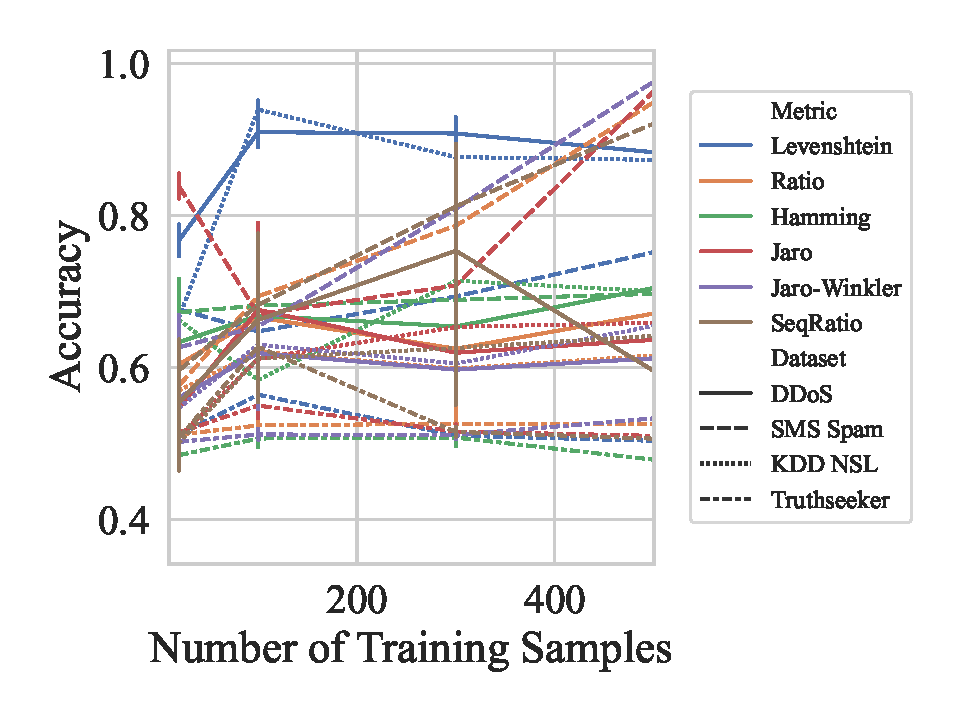
\includegraphics[width=.45\textwidth]{figs/combined/string_metric_vs_accuracy.pdf}
        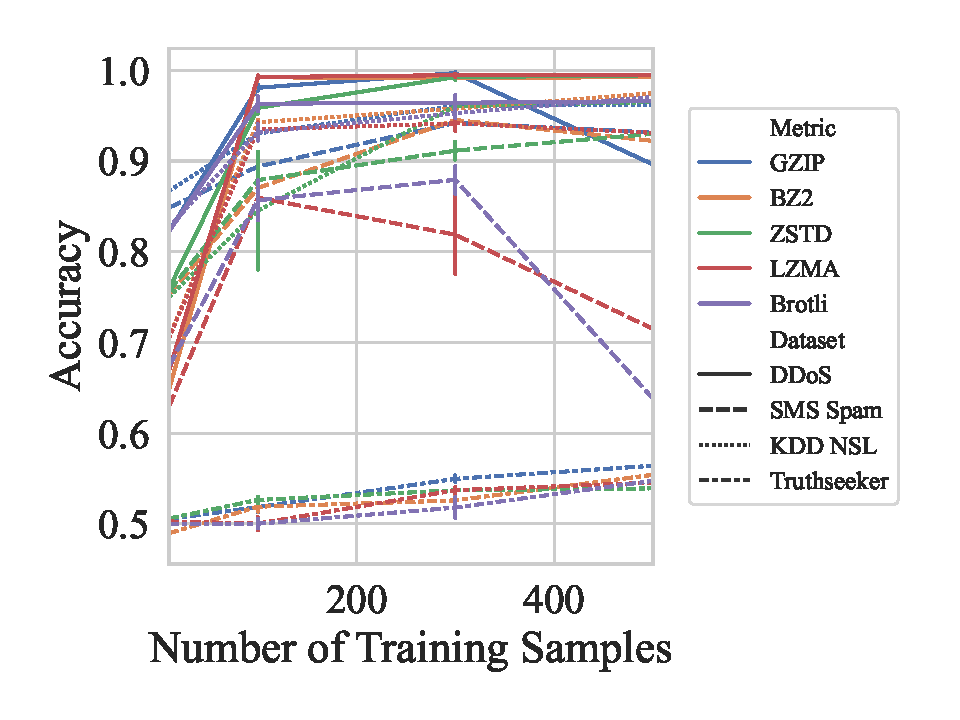
\includegraphics[width=.45\textwidth]{figs/combined/compressor_metric_vs_accuracy.pdf}
    \end{subfigure}
    
    \begin{subfigure}[htb]{\textwidth}
        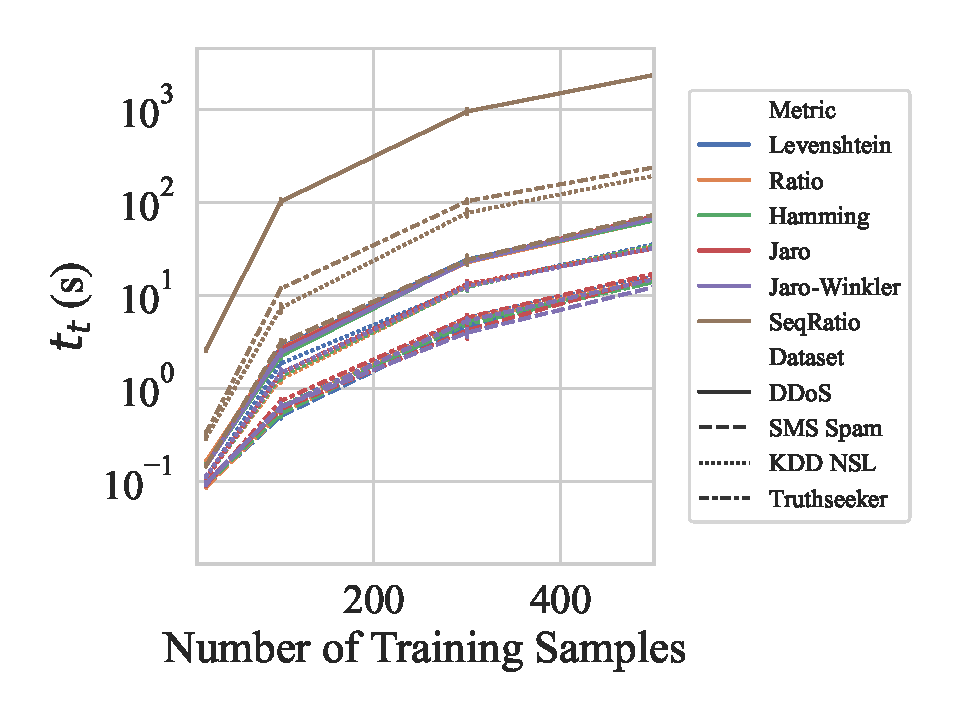
\includegraphics[width=.45\textwidth]{figs/combined/string_metric_vs_train_time.pdf}
        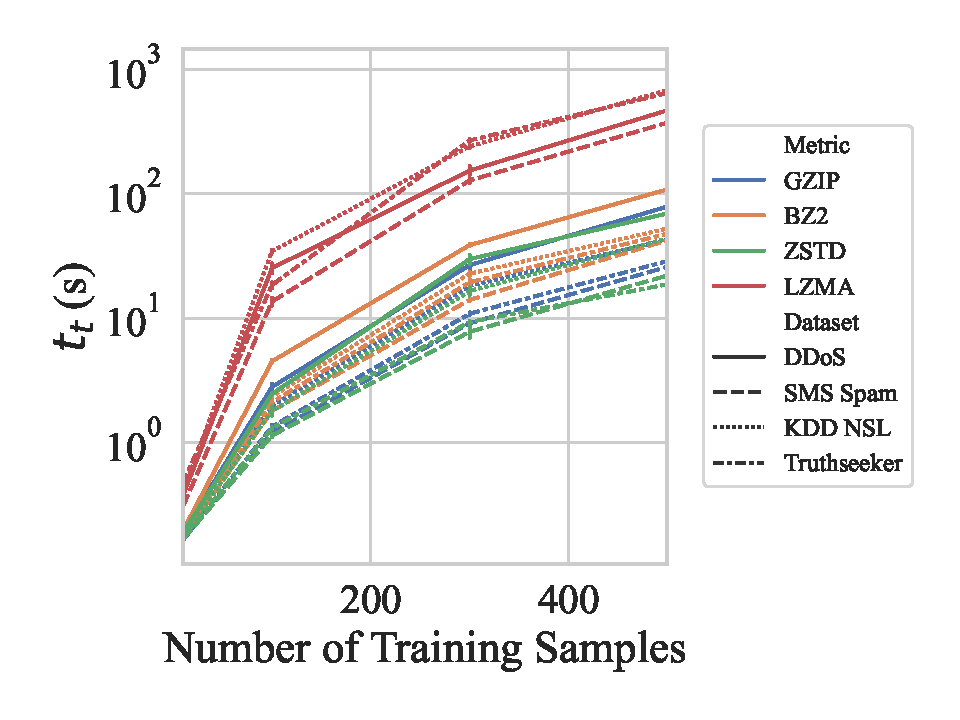
\includegraphics[width=.45\textwidth]{figs/combined/compressor_metric_vs_train_time.pdf}
    \end{subfigure}
   
    \begin{subfigure}[htb]{\textwidth}
        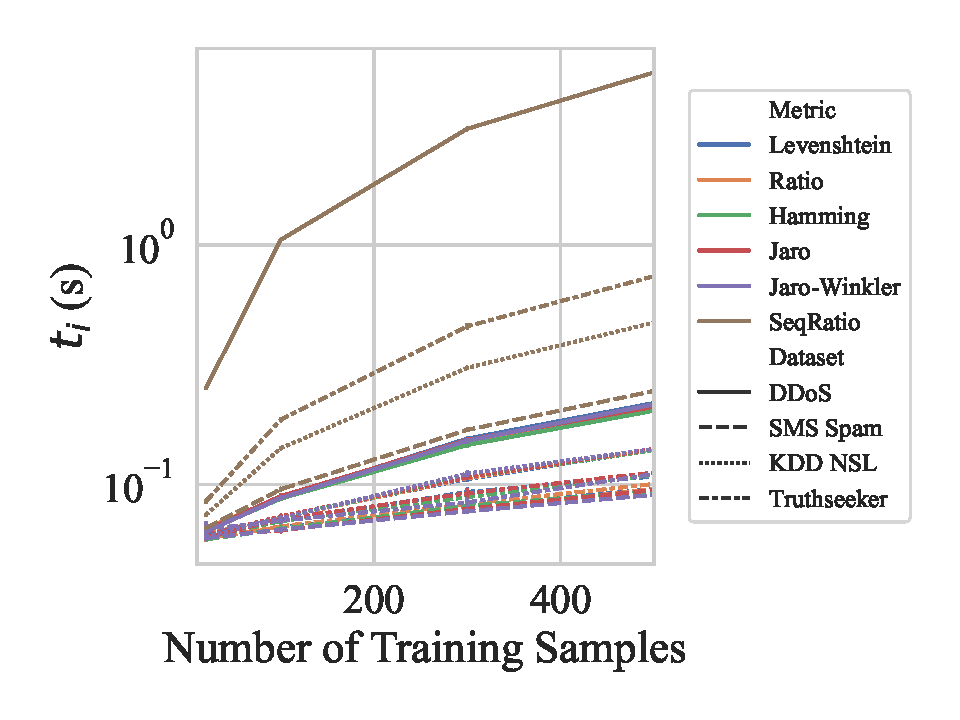
\includegraphics[width=.45\textwidth]{figs/combined/string_metric_vs_predict_time.pdf}
        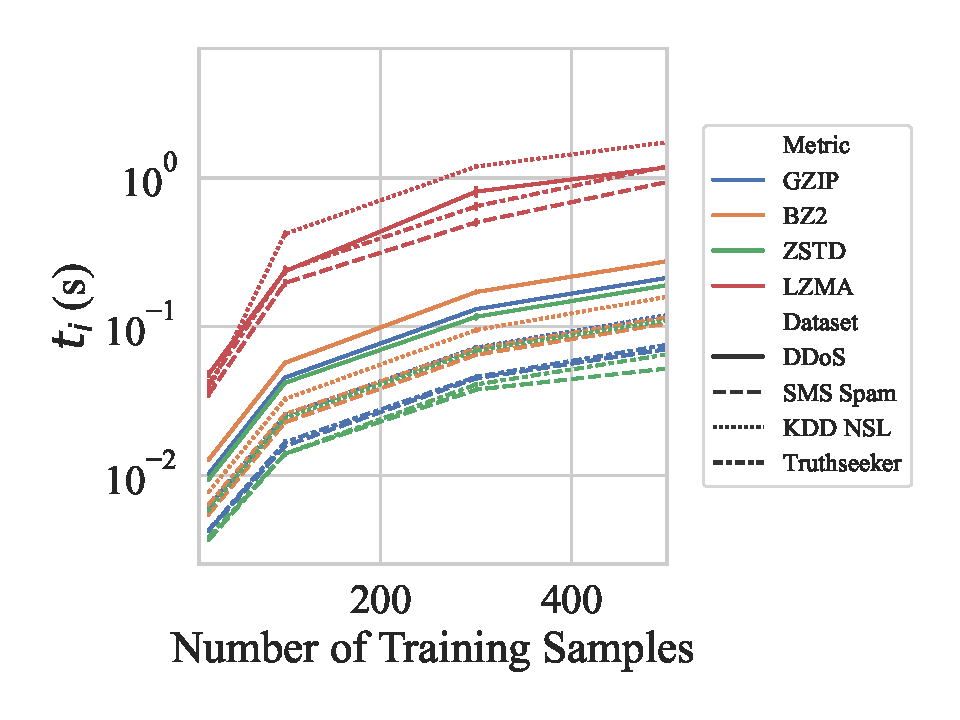
\includegraphics[width=.45\textwidth]{figs/combined/compressor_metric_vs_predict_time.pdf}
    \end{subfigure}
    
    \caption{String-metric based classifier accuracy (top), training times (middle), and inference times (bottom) across many datasets (style), and models. The left column depicts the results from the tested string metrics (see: Section~\ref{string_metrics}) and the right side depicts the results from the modified NCD algorithm using various compressors (see: Section~\ref{compressors})}
    \label{fig:models_summary}
\end{figure*}

Figure~\ref{fig:models_summary} shows the performance of the various classifiers (knn, logistic, SVC) across each of the datasets using various string metrics (left column) and compressors (right column) to calculate NCD. We see that run-times are largely comparable between NCD and various string metrics for both training ($t_t$) and inference ($t_i$). 
However, NCD provides consistently more accurate results with a small number of samples, apart from Levenshtein distance which works quite well with 10s of samples. 
Please note that the training step is only necessary for certain configurations of the KNN algorithm and that the vanilla version proposed by Jiang et. al.~\cite{jiang2022less} can skip this step entirely. However, Figure~\ref{fig:mod_acc} shows that kernelized SVCc and Logistic Regressors can offer improved accuracy over this "untrained" version.
However, As we increase the number of samples, Jaro, Waro-Winkler, and seqratio become more useful for the SMS dataset, but remain unremarkable for the other datasets. Overall, NCD offers superior performance over the tested string metrics since it performs consistently well across all of the datasets. 


\subsection{Effect of Modified NCD Algorithm}

\begin{figure*}[htb]
    \centering
    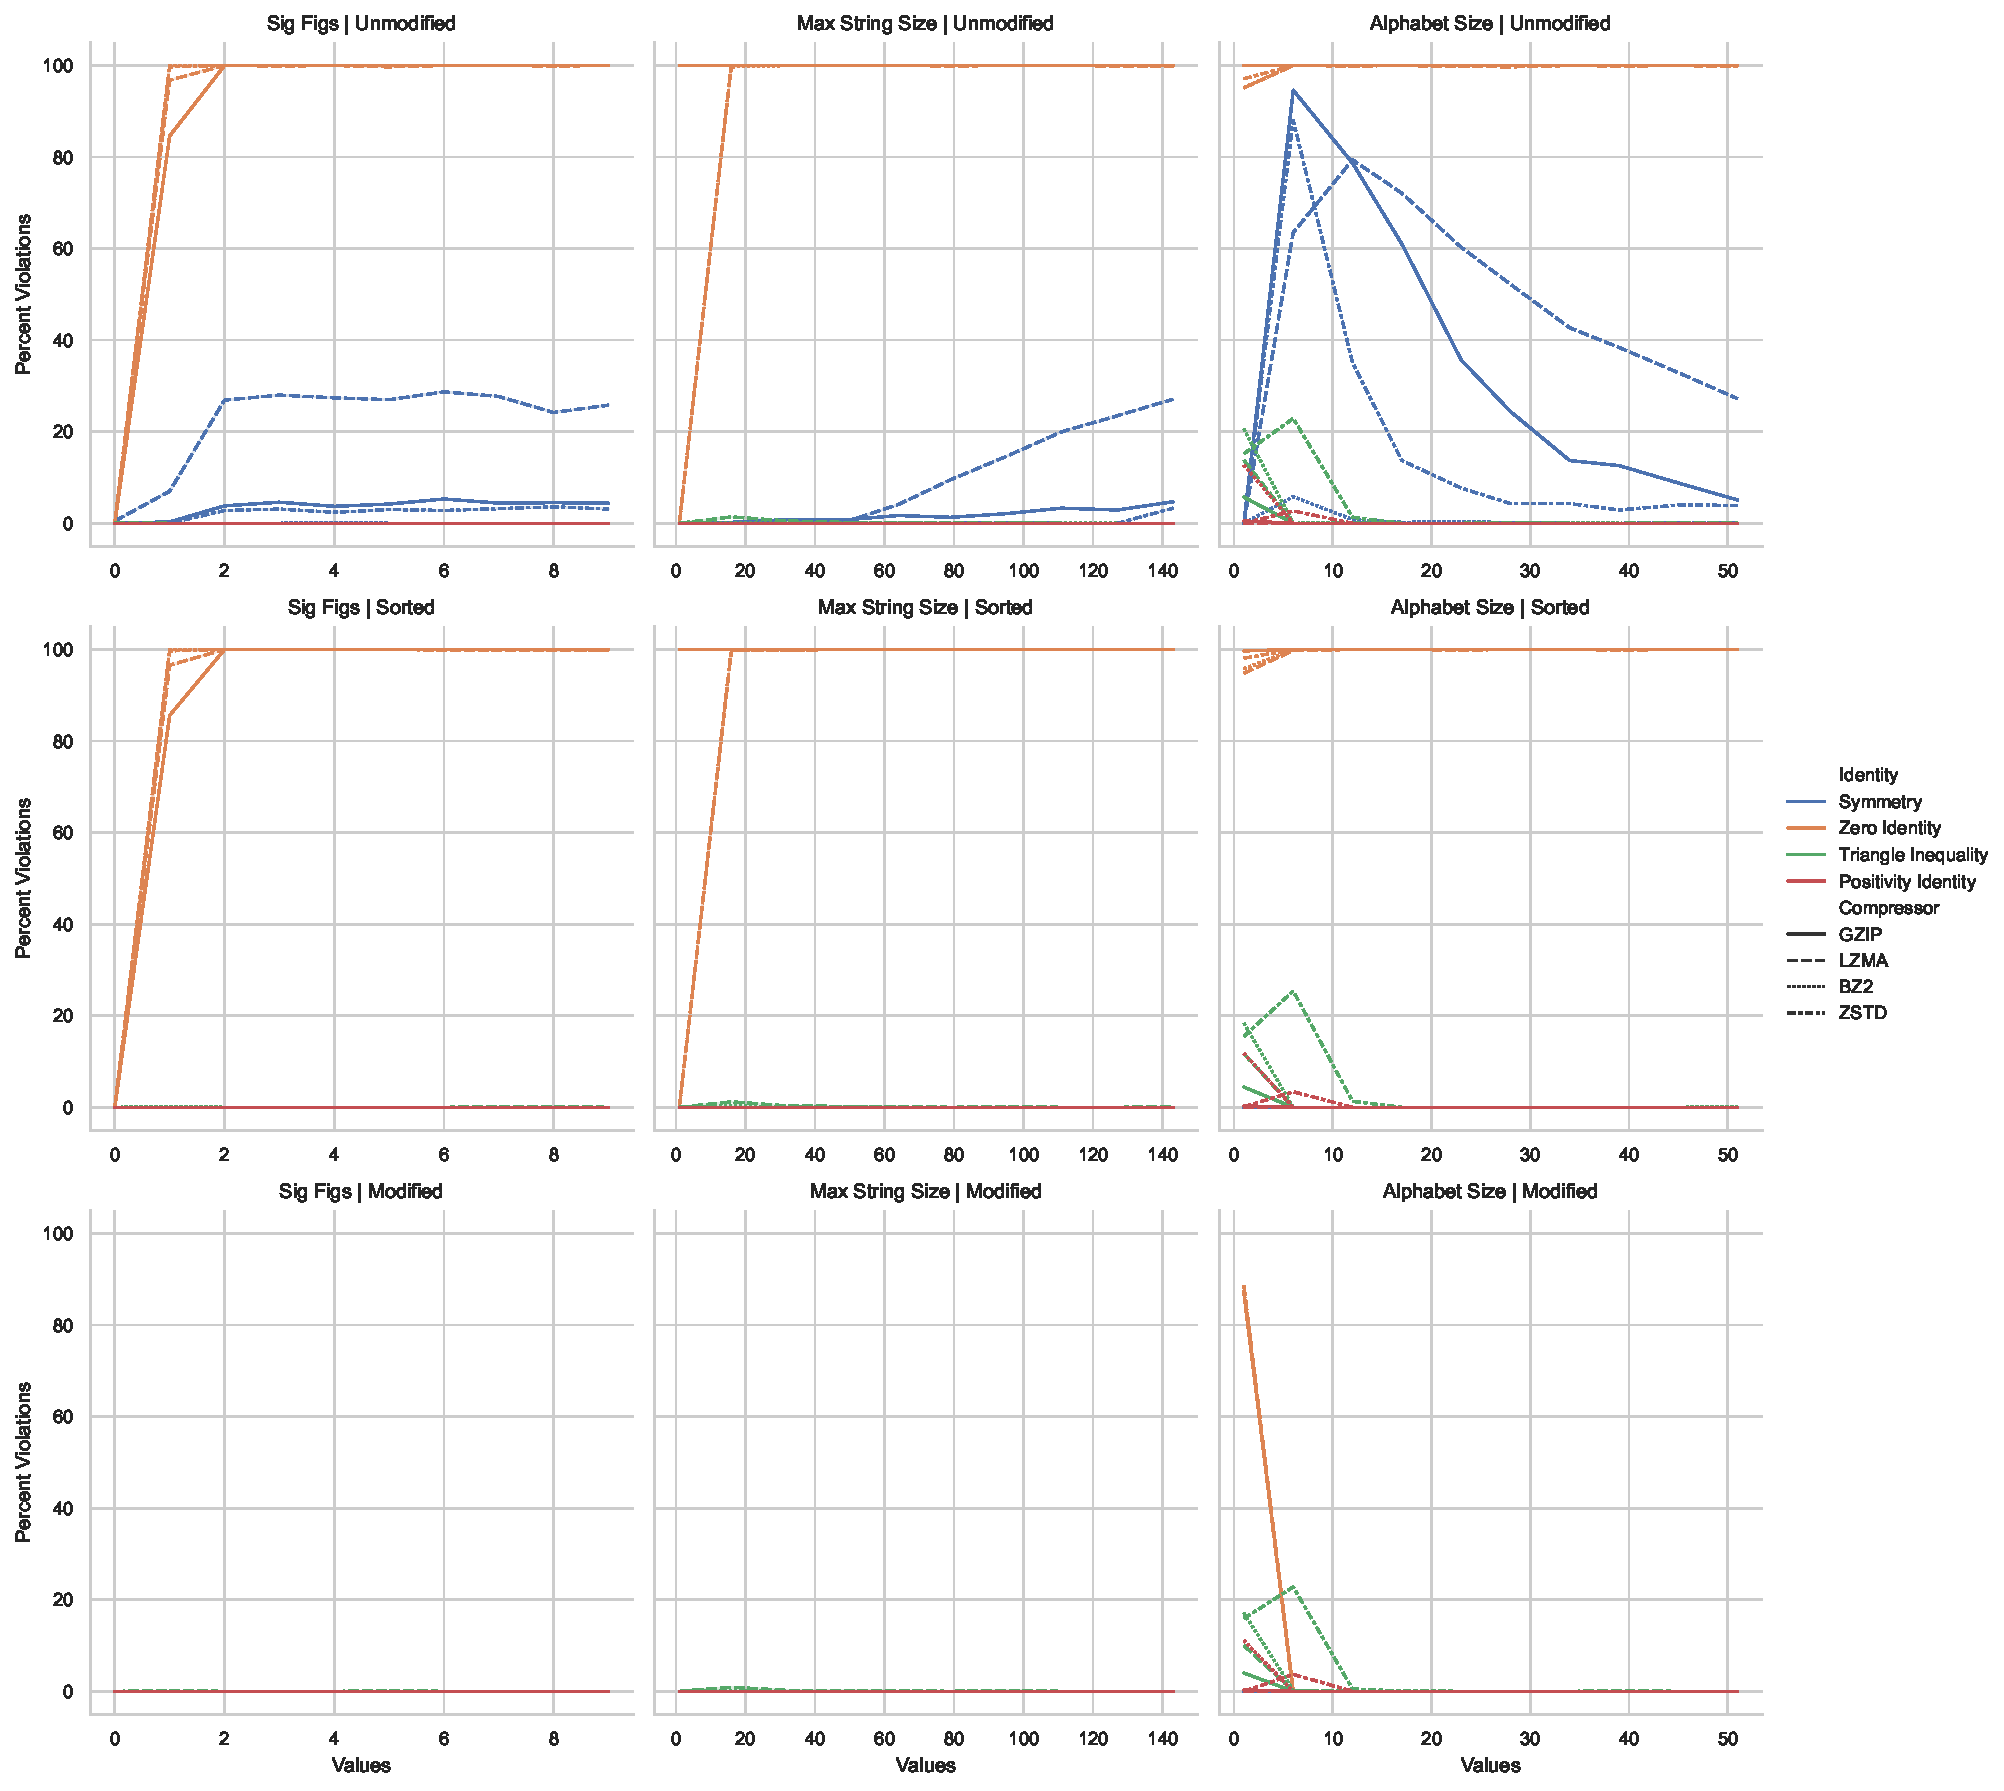
\includegraphics[width=\textwidth]{images/results.pdf}
    \caption{
    Percentage of examples found that violate the assumptions outlined in Section~\ref{metric_spaces} using the vanilla (Algorithm~\ref{alg:vanilla}, top row), assumed symmetry (Algorithm~\ref{alg:assumed_symmetry}, middle row), and modified (Algorithm~\ref{alg:modified}, bottom rows) algorithms on 100 thousand random strings without checking for the special case of $x=y$ (middle row) and using an if statement to check that special case (bottom row). 
    \textit{Sig Figs} refers to the number of significant figures. \textit{Max String Size} and \textit{Max Alphabet Size} refer to the number of characters and the number of unique characters respectively. 
    Unless otherwise specified by the x-axis in an individual plot, \textit{Max String Size}, \textit{Max Alphabet Size}, and \textit{Sig Figs} were all 144 characters (the character limit of a ``tweet''), 52 letters (upper and lower case English letters), and 10 significant figures. Each colour corresponds to a different identity as defined in Section~\ref{metric_spaces} and each line marker corresponds to a different compression algorithm as outlined in Table~\ref{tab:compression_algorithms}.
    }
    \label{fig:mod_assumptions}

\end{figure*}

\begin{figure*}[htb]
    \centering
    \begin{subfigure}[htb]{\textwidth}
        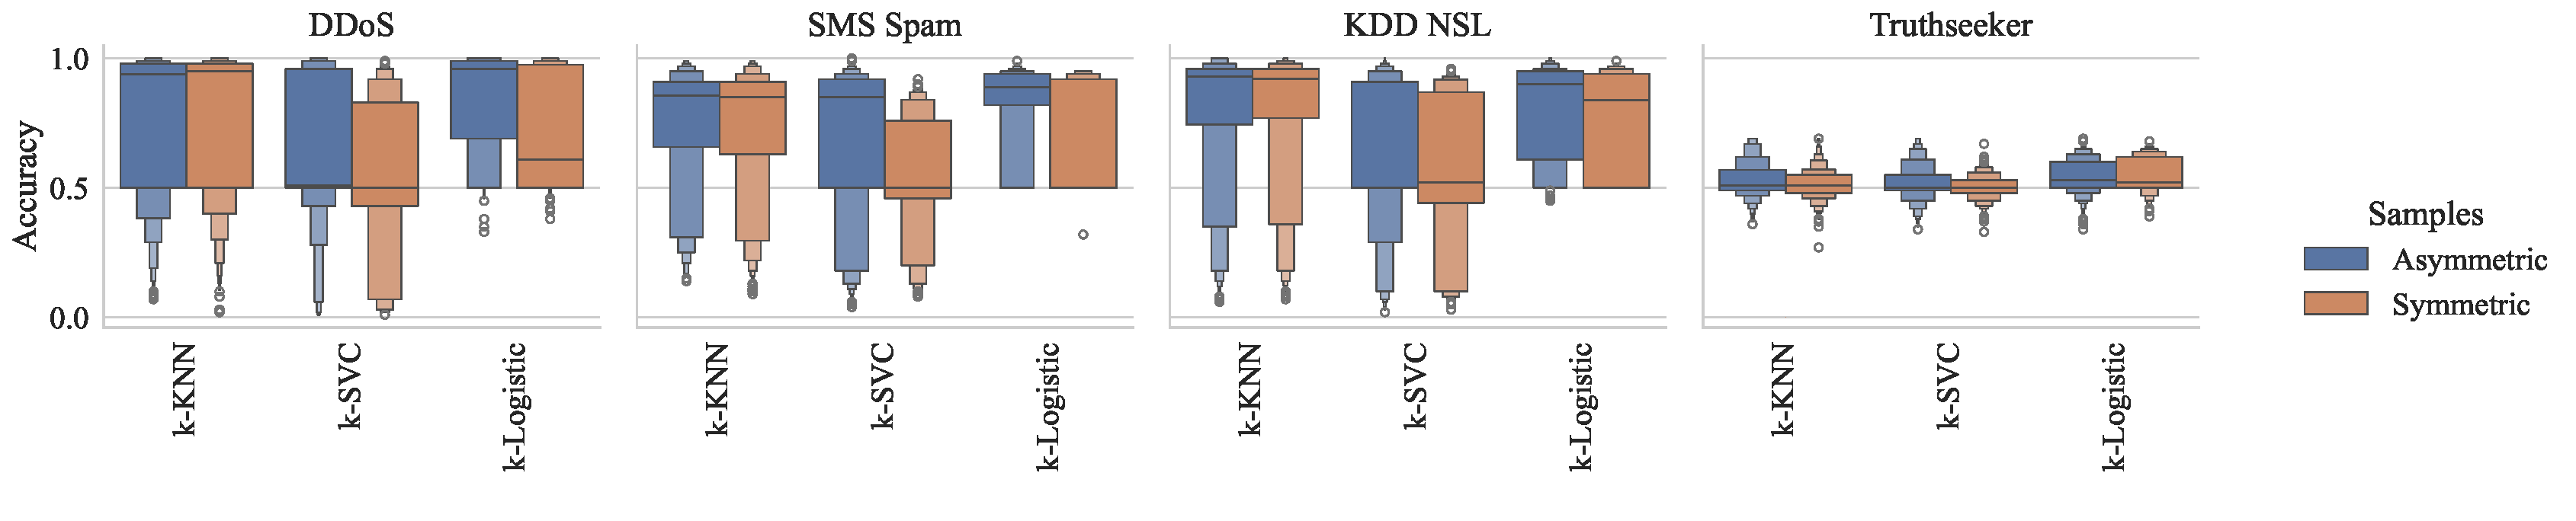
\includegraphics[width=\textwidth]{figs/combined/symmetric_models_vs_accuracy.pdf}
        \caption{Accuracy across models and datasets.}
        \label{fig:mod_acc}
    \end{subfigure}
    \begin{subfigure}[htb]{\textwidth}
        \centering
        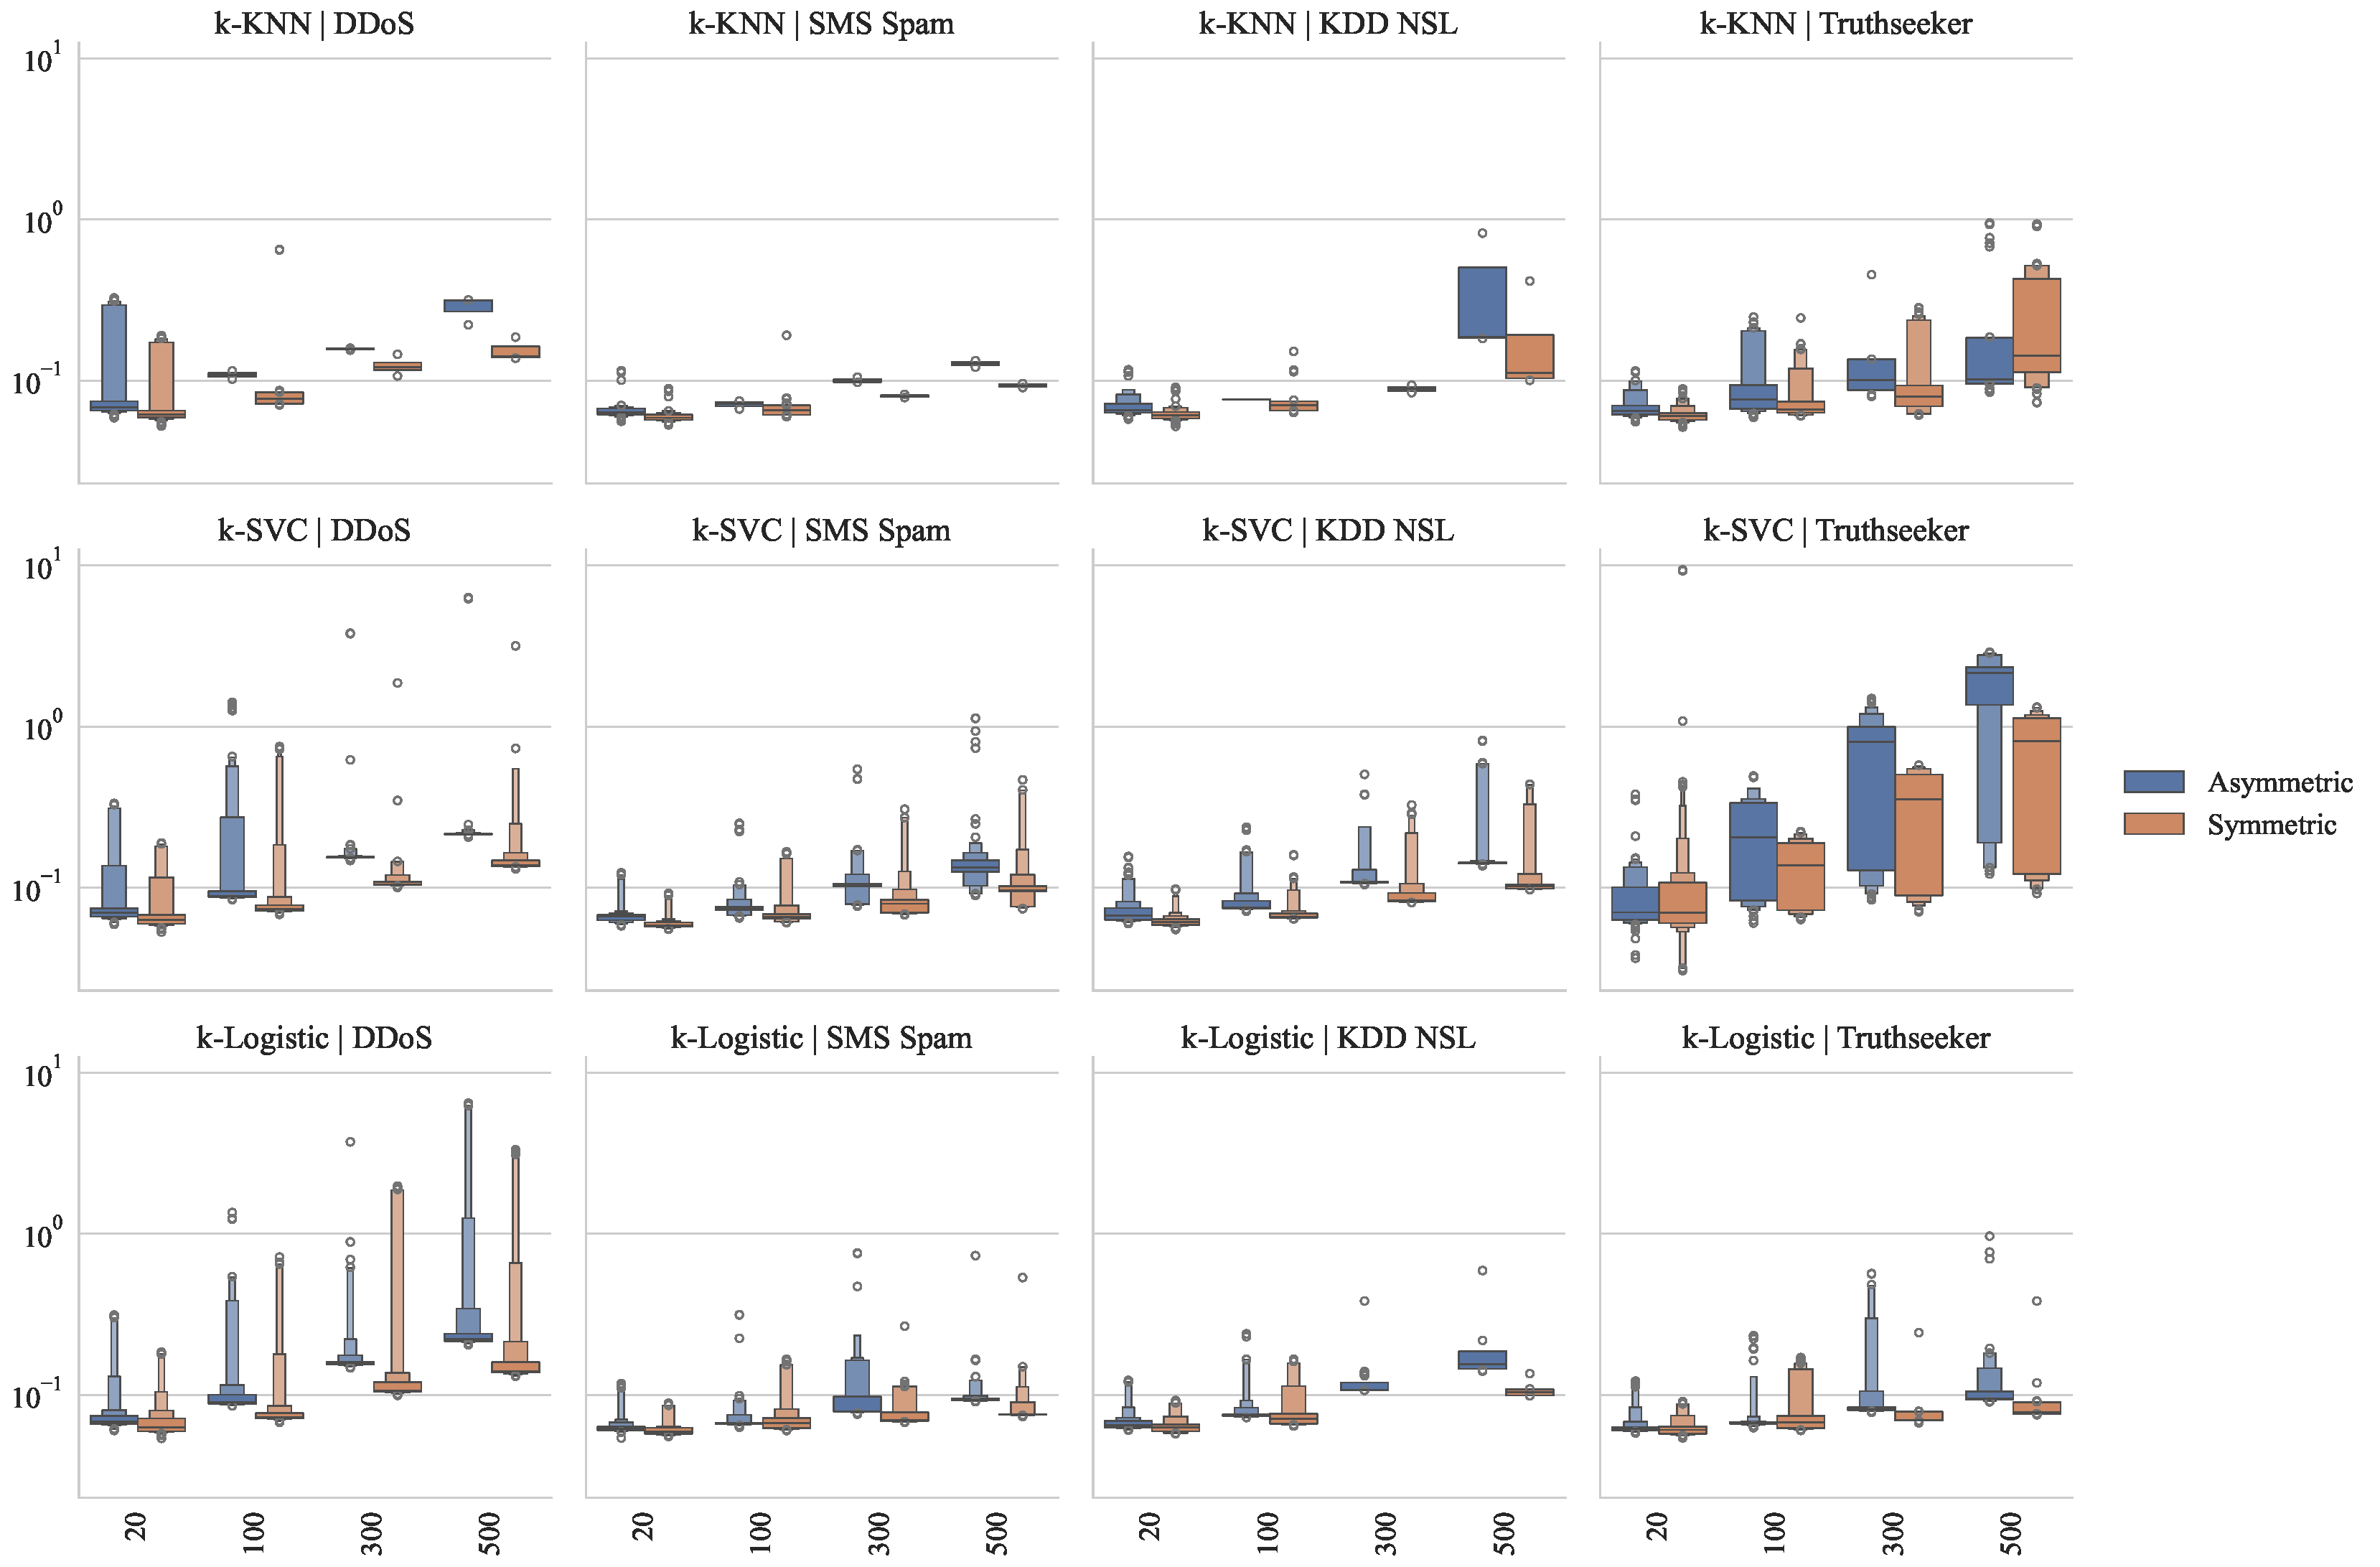
\includegraphics[width=\textwidth]{figs/combined/symmetric_models_vs_train_time.pdf}
        \caption{Training Times across models and datasets.}
        \label{fig:mod_train_time}
    \end{subfigure}
    \begin{subfigure}[htb]{\textwidth}
        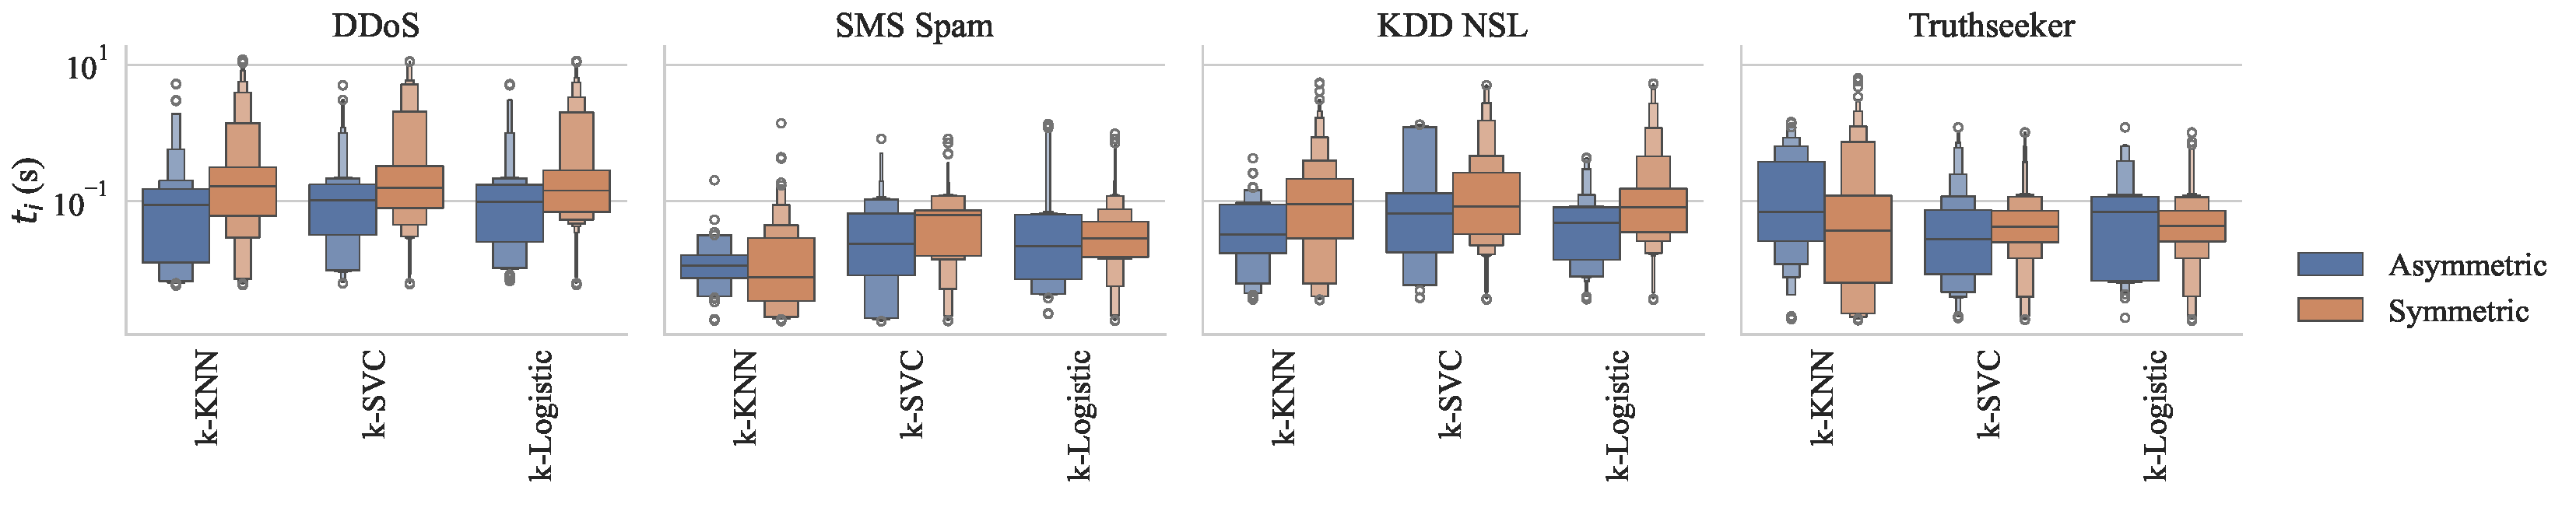
\includegraphics[width=\textwidth]{figs/combined/symmetric_models_vs_predict_time.pdf}
        \caption{Prediction Times across models and datasets.}
        \label{fig:mod_pred_time}
    \end{subfigure}
    \caption{Kernelized classifier inference times across many datasets, and models while examining the effect outlined in Algorithm~\ref{alg:modified}. Each column corresponds to a different dataset and each row corresponds to a different performance metric (accuracy, training time per sample, and inference time per sample), the value of which is on the y-axis. The x-axis in each plot corresponds to a classifier type and the colour conveys whether the modified NCD function  was used (orange, Algorithm~\ref{alg:modified}) or not (blue, Algorithm~\ref{alg:vanilla}).}
    \label{fig:mod_summary}
\end{figure*}

Figure~\ref{fig:mod_summary} depicts the accuracy (top), training time per sample (middle), and inference time per sample (bottom) for each the vanilla (denoted in orange) and the modified algorithm (see: Algorithm~\ref{alg:modified}, denoted in blue). 
The accuracy of the modified algorithm is fairly consistent with the unmodified version. 
In practice, the model builder would choose the most accurate model, which is consistent across the algorithms and classifiers for each dataset. 
However, the modified version of the algorithm is clearly much faster per sample when constructing the Gram matrix ($t_t$) by reducing the number of distance computations by a factor of 2. 
This comes at the marginal cost of a few hundred milliseconds for each prediction, however, but this could easily be mitigated by skipping the algorithmic modifications during the prediction step and handle the problem of negative distances at run-time, depending on the particular application. 
Overall, it is clear that this modified version of NCD offers significant run-time improvements while costing nothing in terms of accuracy. 
Additionally, by running the vanilla version during prediction and using the modified version if and only if the Gram matrix is calculated, these downsides can be avoided entirely. 
However, that may produce Gram matrices that are incompatible with other tooling or models (see: Figure~\ref{fig:mod_assumptions}, middle row), most of these are mitigated with the proposed modifications (see: Figure~\ref{fig:mod_assumptions}, bottom row). 
However, two classes of counterexamples remain. 
The first occurs with very short strings
$NCD("ABB", BBBB) =0$ because the marginal length associated with the repeated ``BB'' token happens to be the exact length as the marginal length associated with the token ``A''. 
This second occurs for the triangle inequality. 
Letting $x =AACAABC, y = AA,
z=AAA$, we find that $NCD(x,y) \approx .26$ while $NCD(x,z) + NCD(z,y) \approx .23$, but it's not clear that this is a problem in the theory. Including the string ``AAA'' provides additional context that ``AA'' may have a distinct meaning apart from ``A'' repeated twice which is why the distance of the sum \textit{is} less than the distance between $x$ and $z$. Additionally, it doesn't seem to be a problem in practice. 
As the max string size or the maximum alphabet size is increased, these problems quickly disappear(see: Figures~\ref{fig:mod_assumptions}~and~\ref{fig:mod_acc}).




\subsection{Database Condensing Methods}

\begin{figure*}[htb]
    \centering
    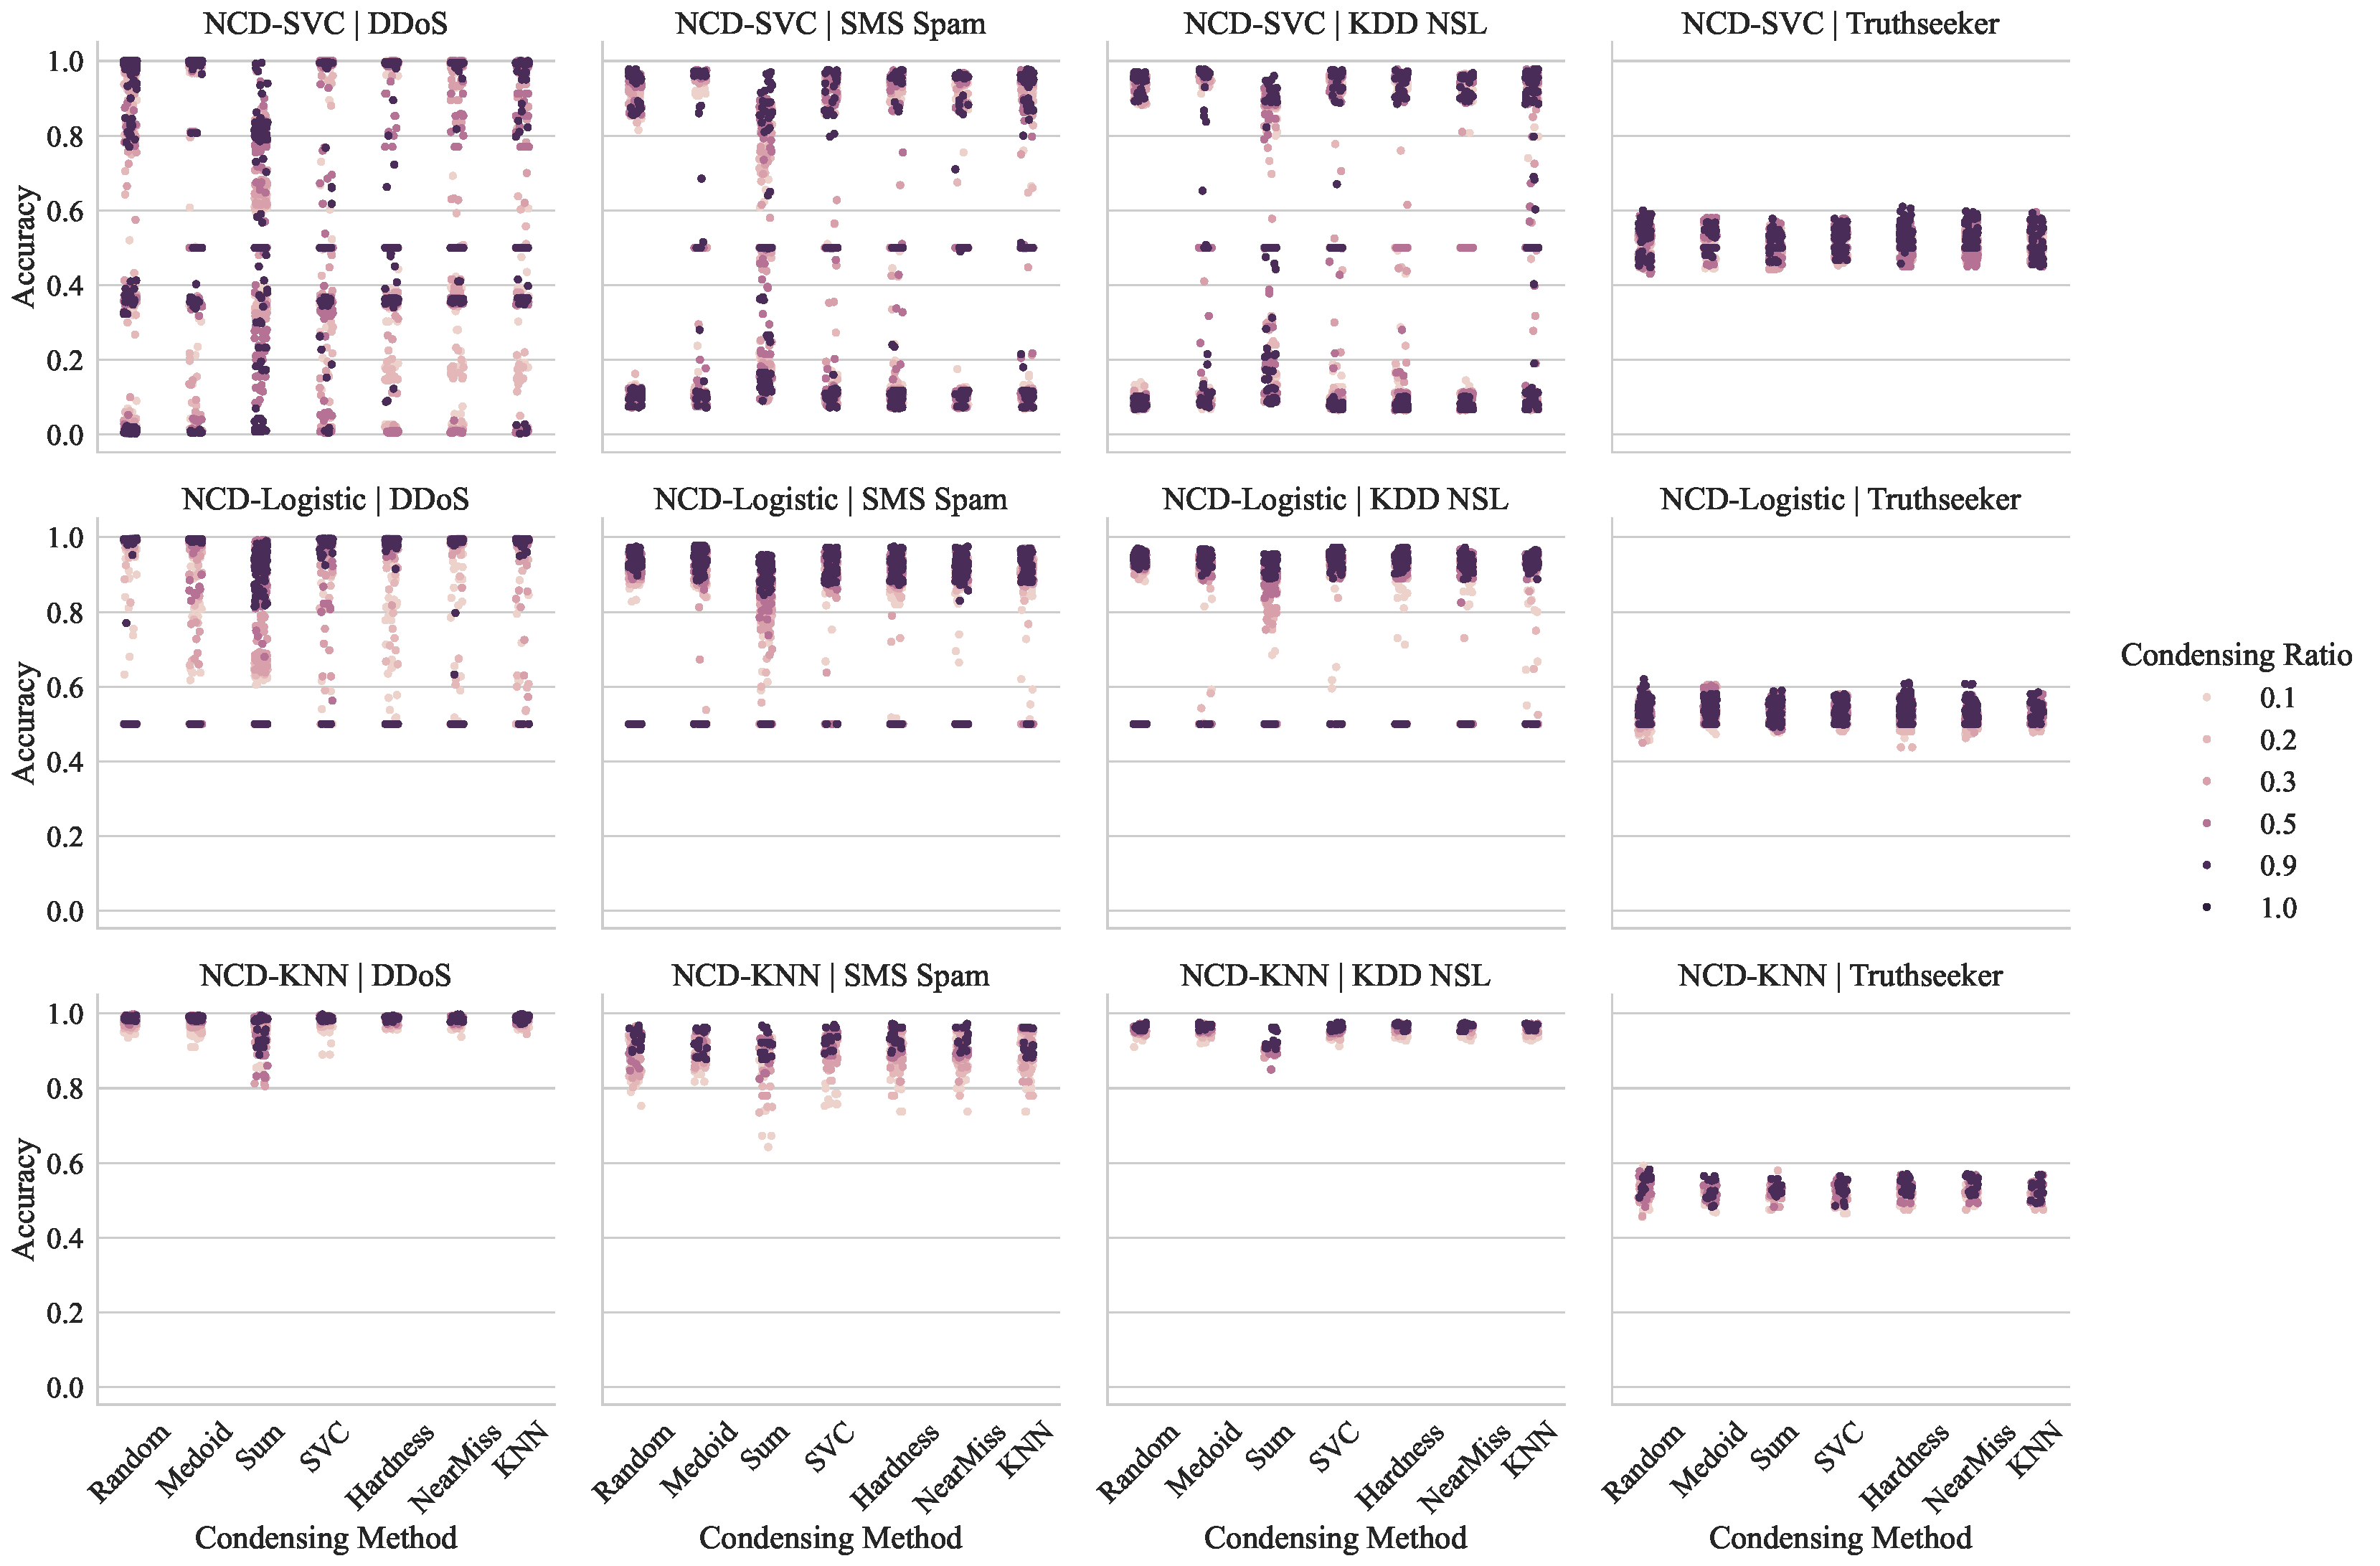
\includegraphics[width=\textwidth]{figs/combined/condensing_ratio_vs_accuracy.pdf}
    \caption{Accuracy across models (rows) and datasets (columns) where the hue represents the condensing ratio (percentage of samples in training database used for prediction) for each condensing method (x-axis). }
    \label{fig:condense_acc_ratios}
\end{figure*}

\begin{figure*}[htb]
    \begin{subfigure}[htb]{\textwidth}
        \centering
        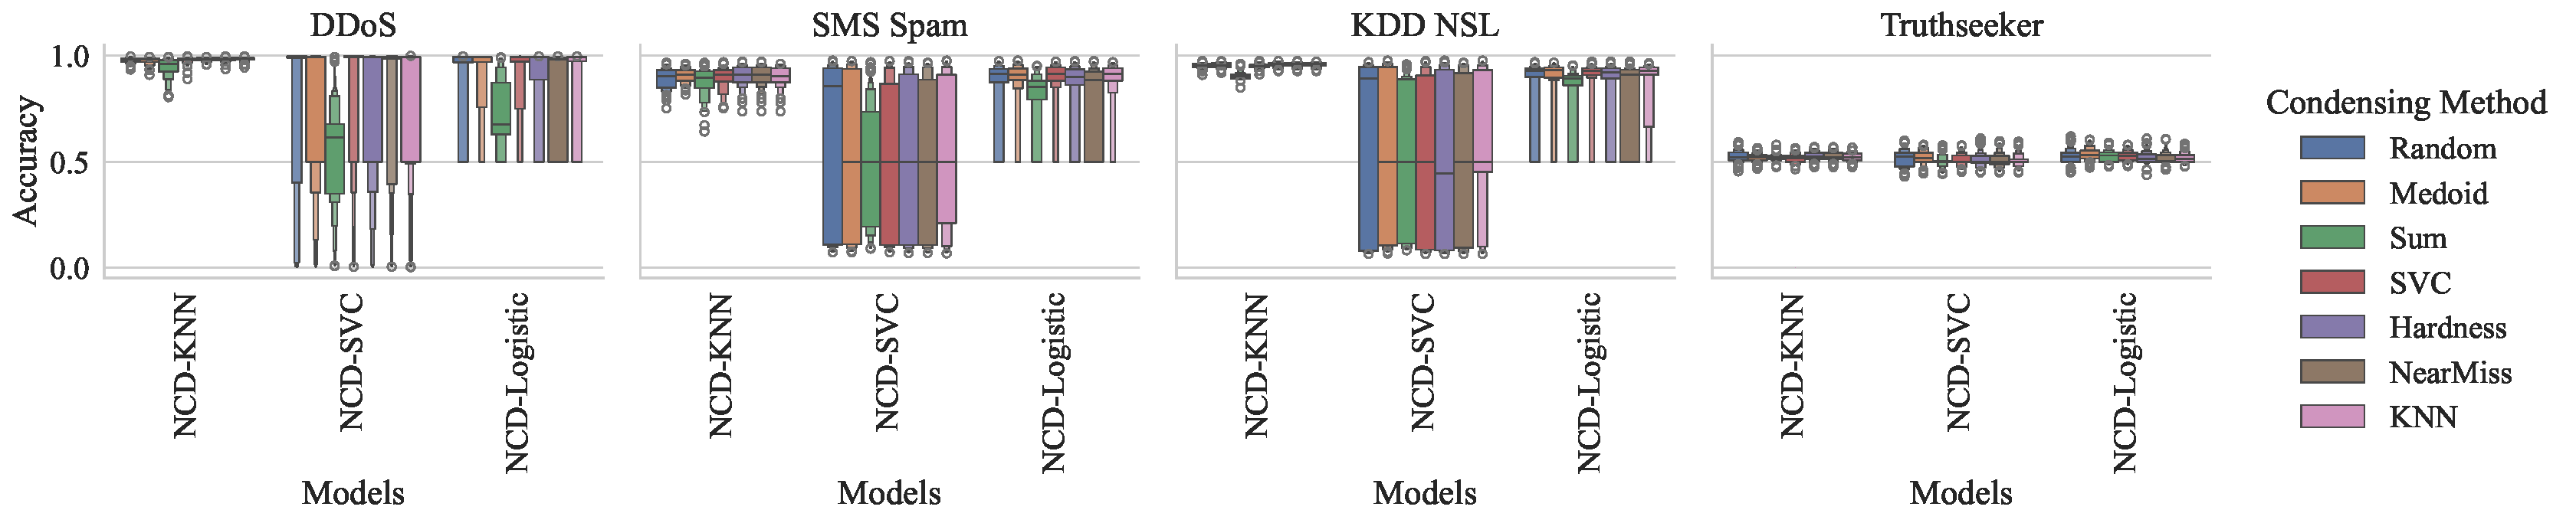
\includegraphics[width=\textwidth]{figs/combined/condensing_methods_vs_accuracy.pdf}
        \caption{Training Times across models and datasets.}
        \label{fig:condense_acc}
    \end{subfigure}
    \begin{subfigure}[htb]{\textwidth}
        \centering
        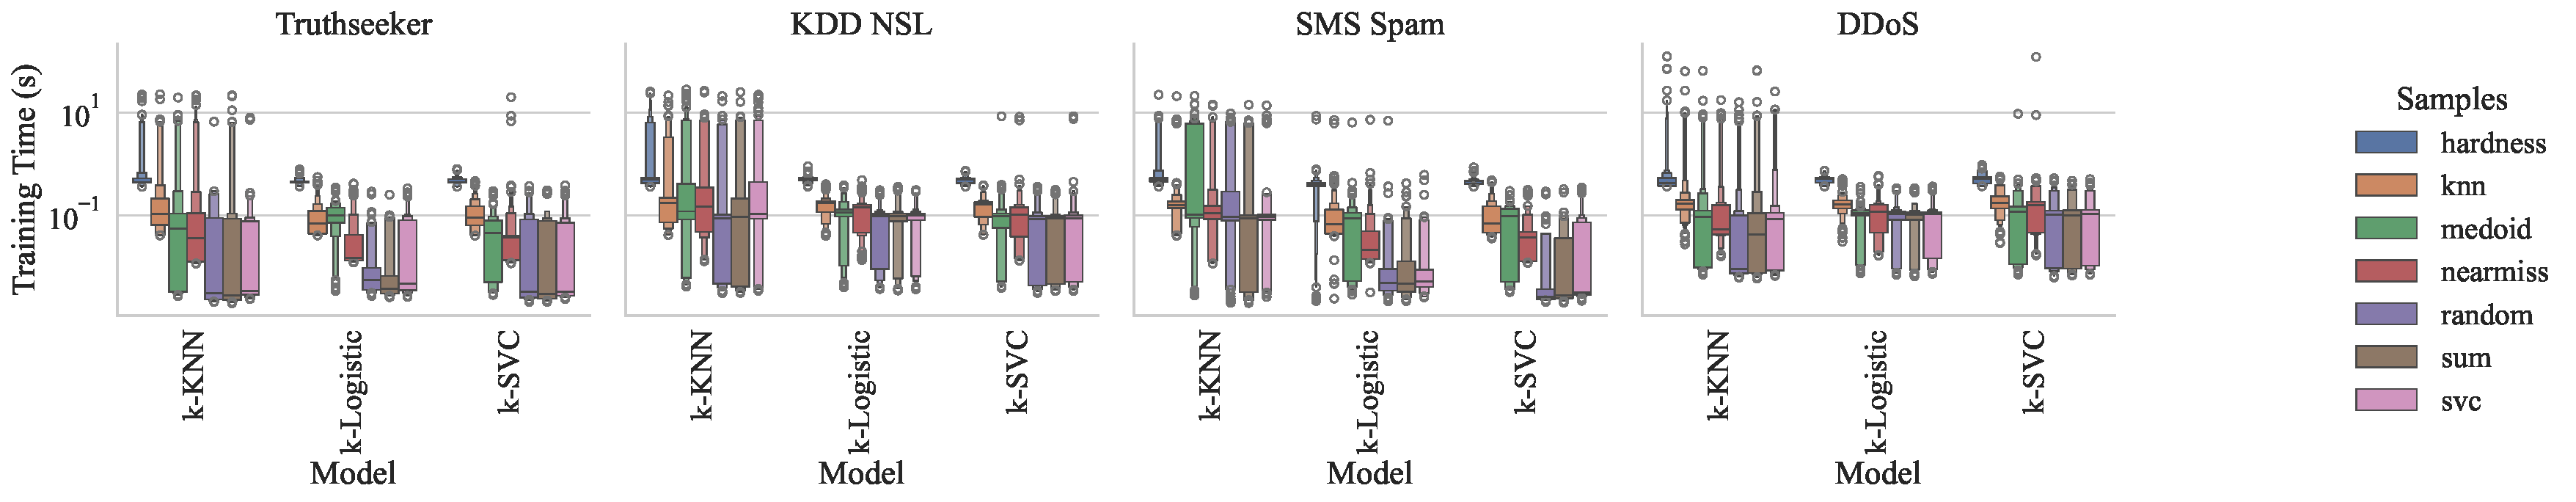
\includegraphics[width=\textwidth]{figs/combined/condensing_methods_vs_train_time.pdf}
        \caption{Training Times across models and datasets.}
        \label{fig:condense_train_time}
    \end{subfigure}
    \begin{subfigure}[htb]{\textwidth}
        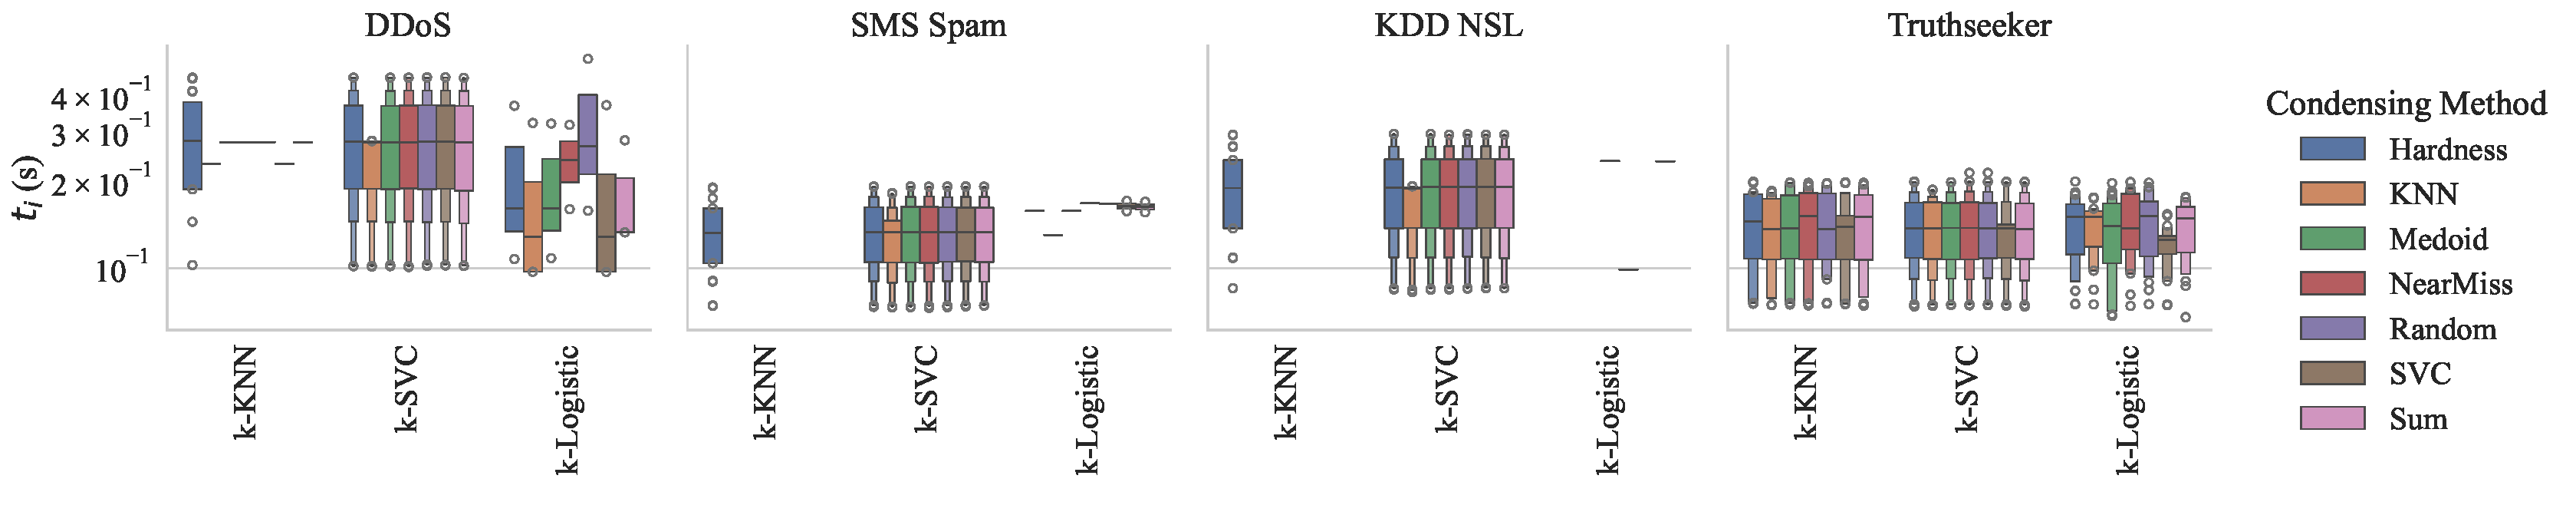
\includegraphics[width=\textwidth]{figs/combined/condensing_methods_vs_predict_time.pdf}
        \caption{Prediction Times across models and datasets.}
        \label{fig:condense_pred_time}
    \end{subfigure}
    \caption{NCD classifier accuracy, inference time per sample ($t_i$), and training time per sample($t_i$). 
    Each column corresponds to a different dataset and each row corresponds to a different performance metric, the value of which is on the y-axis. 
    The x-axis in each plot corresponds to a classifier type and one one colour is assigned to each condensing method.}
    \label{fig:condense_summary}
\end{figure*}

Figure~\ref{fig:condense_acc_ratios} depicts the accuracy across all models, datasets, and condensing ratios while Figure~\ref{fig:condense_summary} depicts the run-time requirements of various condensing methods. 
For each condensing ratio (e.g. percentage of training samples used during prediction), 128 trials were conducted to tune the hyper-parameters of each of the tested models using a variety of methods (see: Section~\ref{condensing_methods} and Figure~\ref{fig:condense_summary}). 
However, the run-time improvements are obvious since the distributions of training times and inference times ($t_t, t_t$ respectively) is effectively the same in both Figures~\ref{fig:condense_summary} and \ref{fig:mod_summary}. That is the condensing methods themselves are fast enough to more than overcome their run-time downsides. 
While it is clear from the former that NCD is quite capable of performing very well on even a small number of samples since the distribution in accuracy does not seem to rely on the compression ratio (see: Figure~\ref{fig:condense_acc_ratios}) and that none of the tested condensing methods consistently outperforms random chance (see: Figure~\ref{fig:condense_acc} meaning this stage is probably unnecessary in practice and that any random subset of samples will be ``good enough''. 

\vspace{-1em}
\section{Considerations}
\label{considerations}
While the proposed algorithm (see:~\ref{alg:modified}) does improve upon certain edge cases outlined in Section~\ref{pseudometric}, the examined condensing methods (see: Section~\ref{condensing}) do not improve upon models trained on samples selected by random chance (see:~\ref{fig:condense_acc}). However, the resulting lack of negative distances allows NCD to be used as part of a kernelized classifier (see: Figures~\ref{fig:condense_acc}~and~~\ref{fig:condense_acc_ratios} to great effect. 
By assuming and enforcing symmetry using the method outlined in Algorithm~\ref{alg:modified}, the training step can be significantly improved.
However, the vanilla NCD-KNN proposed by Jiang et. al.~\cite{jiang2022less} remains an effective choice if the training step is deemed too expensive for the chosen applications.
Here, the authors would like to note the borderline performance of all metrics on the Truthseeker dataset--- both NCD and more traditional distance measures. However, this is on par with the performance from the original authors~\cite{truthseeker}. To the best knowledge of the authors, most content on the platform formerly known as Twitter is simply indistinguishable from bot-generated spam--- using any known distance metric.


\section{Conclusion}
It is clear from Figure~\ref{fig:mod_summary} that our algorithm is superior to the method proposed by Jiang et. al. when applied used a distance measure for kernelized classifiers. By preemptively handling cases that would result in negative values for distance (thus violating the Non-negativity identity) and sorting the inputs, this modified NCD is guaranteed to behave more like a true metric. 
This allows the model builder to use standard tooling (e.g.~\texttt{scikit-learn},~\texttt{imblearn}) to build classifiers that perform well on an exceedingly small number of samples. The end result is a real-time, client-side classification algorithm that doesn't rely on federation, centralization, or the large scale processing of millions of data points across a global user-base. 
This categorically circumvents poisoning attacks~\cite{biggio_poisoning_2013} since each labelled database is unique to each user. 
Furthermore, this reduces the attack surface of attacks like model inference attacks, database exfiltration attacks, and evasion attacks since a malicious user would need to target the personalised classifier of each user~\cite{biggio_evasion_2013,deepfool,chakraborty_adversarial_2018}. 
While it is known that some attacks are quite transferable~\cite{wang2021enhancing}, this reduces the common attack surface to \textit{only} the samples that are universal across the user base and a new model can be generated trivially by refreshing the page or appending the offending sample to the labelled (training) dataset. 


\label{conclusion}


\bibliographystyle{ieeetr}
\newpage
\bibliography{bibliography}

\end{document}
